\chapter{Proof-of-concept}
\label{ch:Proof-of-concept}


In deze proof-of-concept zal er onderzocht worden of een PWA kan voldoen aan het verwachtingspatroon van een gebruiker van een native applicatie.

Er zal een applicatie ontwikkeld worden waarbij een aangemelde gebruiker een andere persoon kan uitnodigen om een videogesprek te hebben. 

 \section{Analyse}
	 \subsection{Functionele requirements}
	 	\subsubsection{Authenticatie}
		 	\begin{itemize}
			 	\item Als een gebruiker wil ik me kunnen registreren met externe platformen (Facebook, Google, ...) zodat ik minder wachtwoorden hoef te onthouden.
			 	\item Als een aangemelde gebruiker wil ik aangemeld blijven als ik de applicatie sluit zodat ik tijd bespaar door  niet bij elk gebruik te moeten aanmelden.
		 	\end{itemize}
		 	
		 \subsubsection{Bellen}
			  \begin{itemize}
			   	\item Als een aangemelde gebruiker wil ik een 'room' aanmaken waar ik een videogesprek kan starten zodat ik in contact kan blijven met iemand waar ik niet fysiek bij kan zijn.
			   	\item Als een aangemelde gebruiker wil ik eenvoudig een link kunnen kopiëren naar mijn 'room' zodat ik deze kan delen met iemand.
			   	\item Als een aangemelde gebruiker wil ik mijn 'rooms' kunnen beheren.
			   	\item Als een aangemelde gebruiker wil ik een notificatie ontvangen als iemand in mijn 'room' komt.
			  \end{itemize}
	 	
	 	\subsubsection{Gebeld worden}
	 	 \begin{itemize}
				\item Als een gebruiker wil ik, als ik een link van een 'room' ontvang, eenvoudig deelnemen aan een videogesprek.
	 	 \end{itemize}
	
		\subsubsection{Algemeen}
	 		\begin{itemize}
	 			\item Als een gebruiker wil ik de toepassing toevoegen aan het startscherm van mijn toestel zodat ik deze snel kan openen.
	 			\item Als een aangemelde gebruiker wil ik de applicatie kunnen openen zonder internetverbinding zodat ik overal en altijd mijn 'rooms' kan bekijken.
			\end{itemize}
	 
	\subsection{Niet-functionele requirements}
		\begin{itemize}
			\item Als een gebruiker wil ik een video-gesprek kunnen hebben met een zo laag mogelijke vertraging zodat ik geen problemen heb met communiceren.
			\item Als een gebruiker wil ik videogesprekken voeren op een veilige manier zodat niemand informatie kan achterhalen die ik niet publiek wou maken.
		\end{itemize} 
		

\newpage
\section{Design}
		\subsection{Mockup}
					
			Voor er een design gemaakt werd, werden er mockups opgesteld (figuur \ref{fig:mockup}). 
			Aan de hand van deze mockups met weinig detail, kon er snel gestart worden met het ontwikkelen van de functionaliteiten. \autocite{Tate2019}
			\begin{figure}[H]
				\centering
				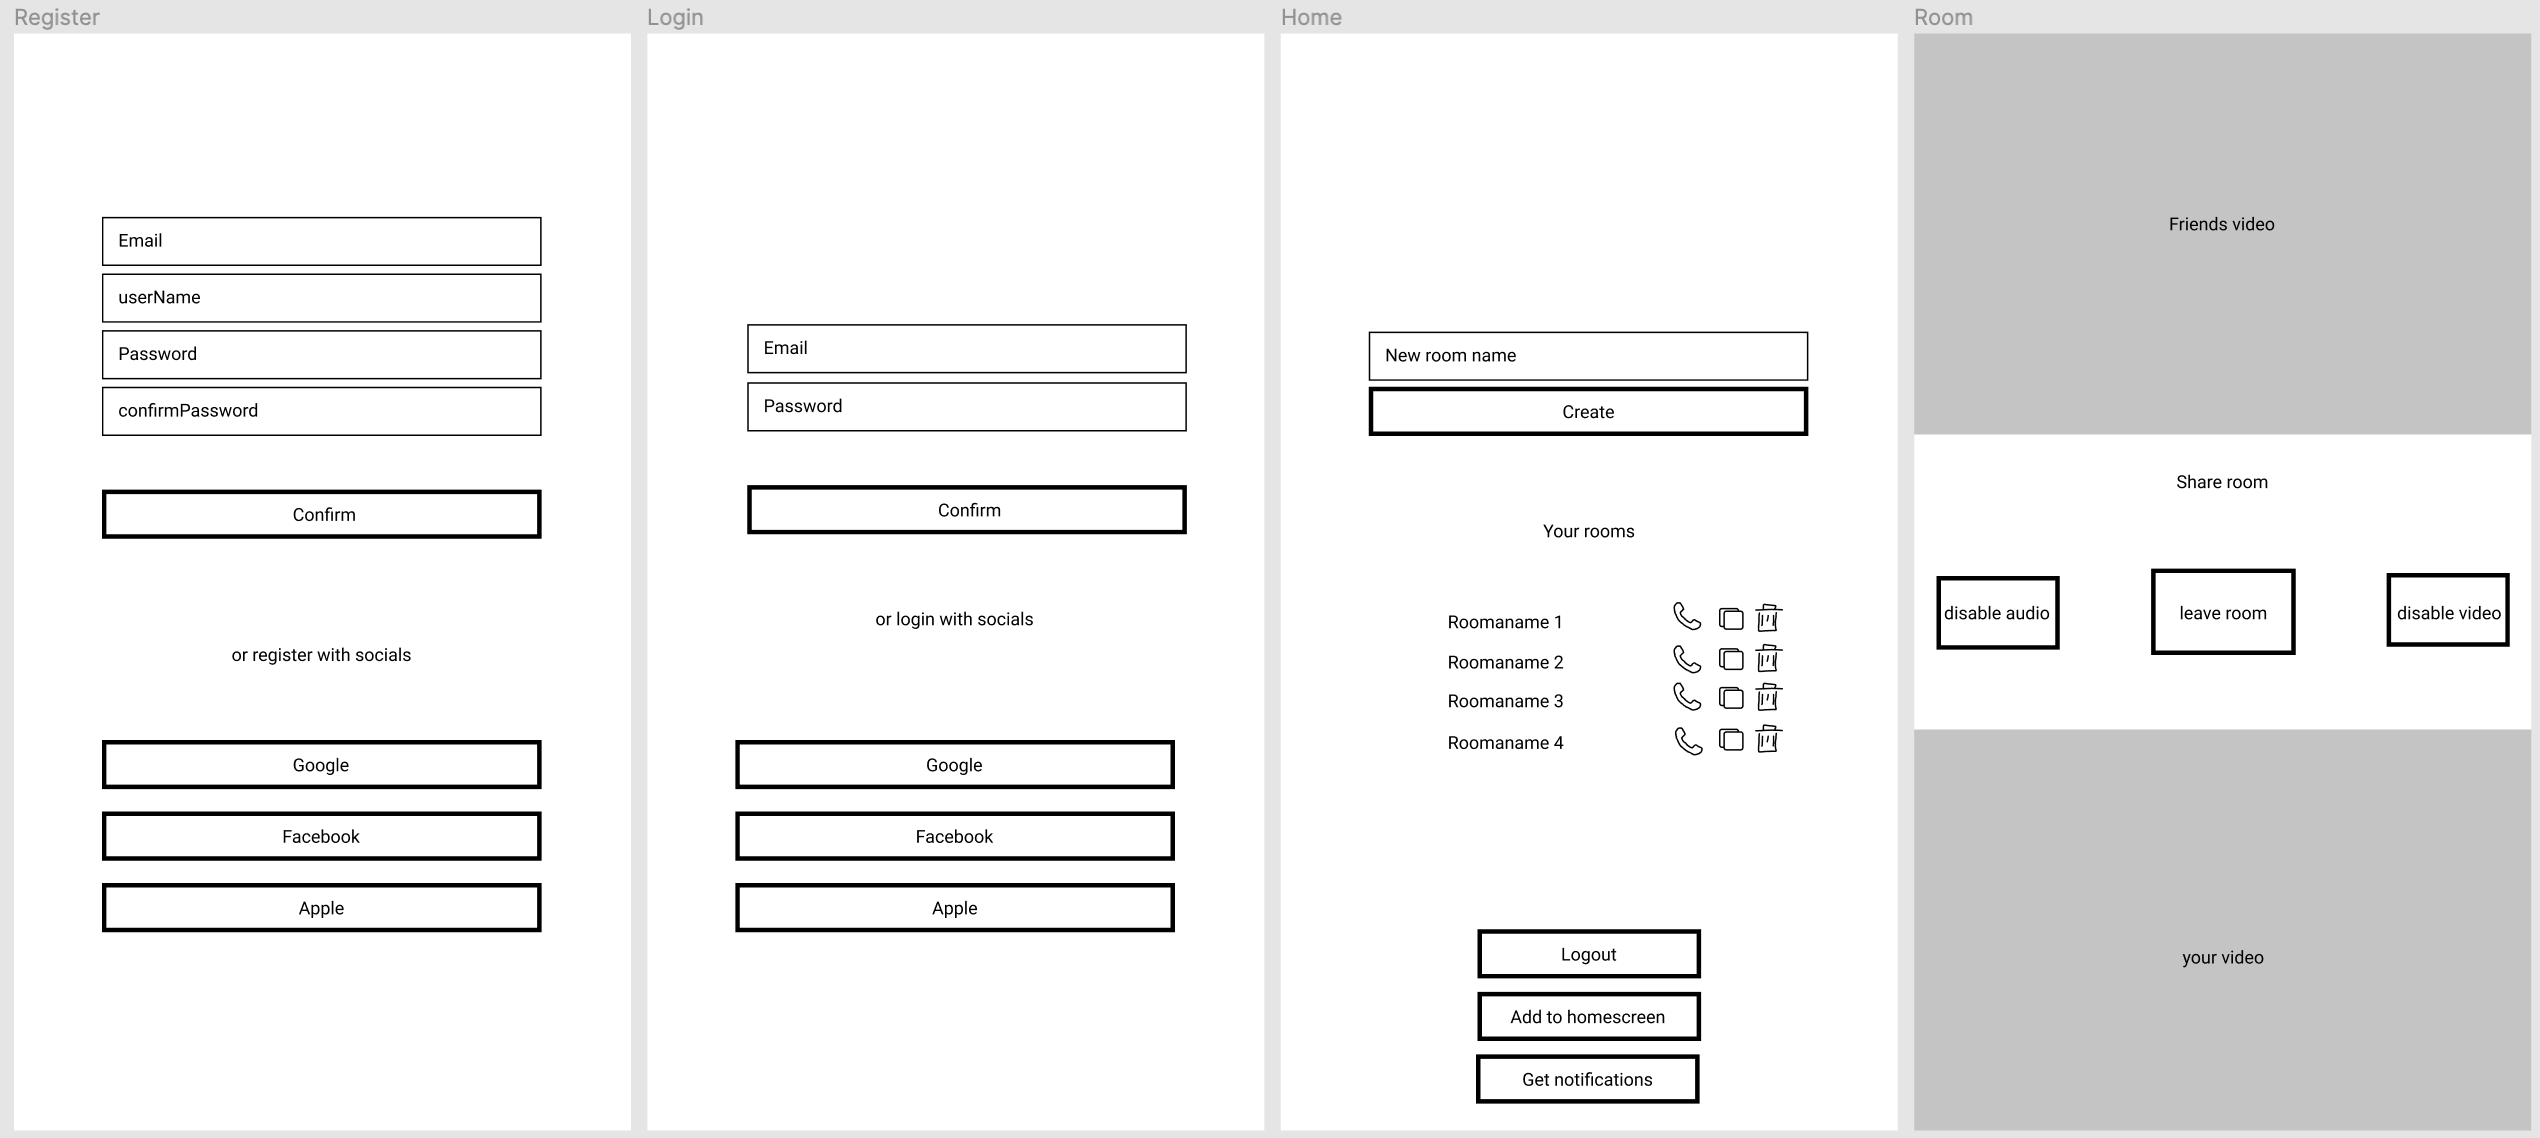
\includegraphics[width=140mm]{./img/mockup-poc.png}{}
				\caption{mockups in Figma}
				\label{fig:mockup}
			\end{figure}
		
		
		\subsection{Prototype}
		
			Vervolgens werd er een klikbaar prototype gemaakt (figuur \ref{fig:design}). In de dit prototype werd de stijl van de applicatie bepaald.
			
			Er werd gekozen om een eenvoudig design te implementeren met illustraties die van \href{https://undraw.co/}{unDraw} verkregen werden.
			
			\begin{figure}[H]
				\centering
				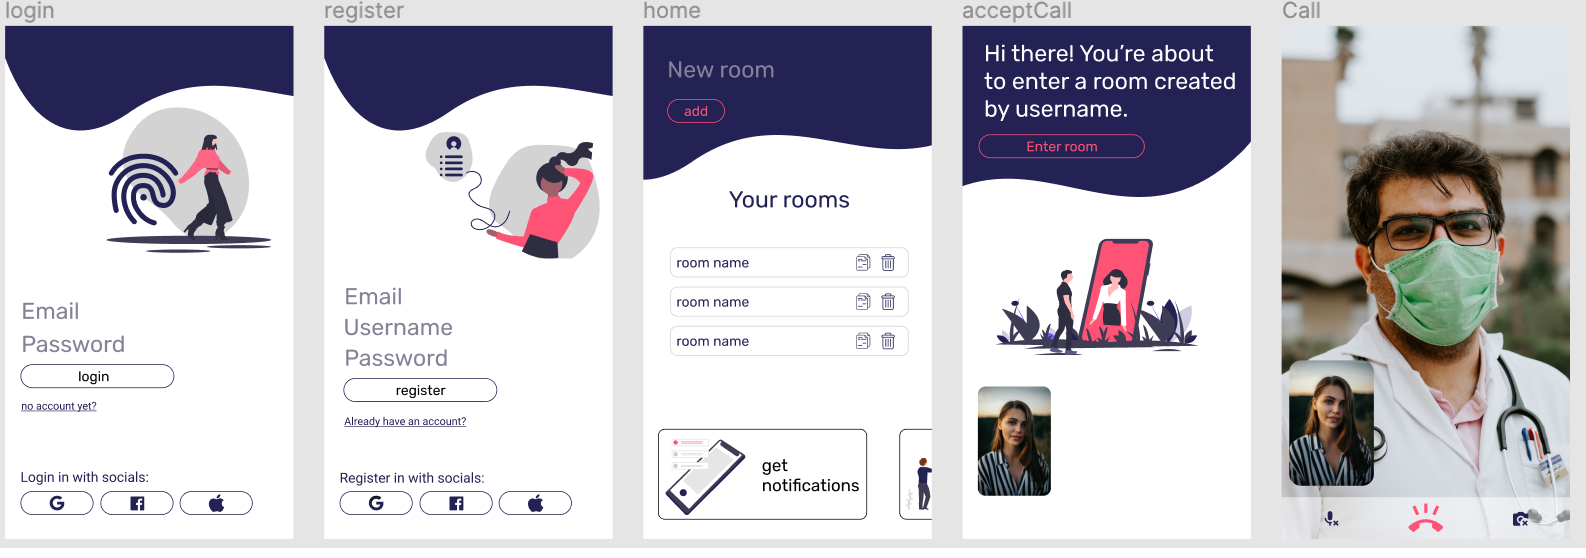
\includegraphics[width=140mm]{./img/prototype-poc.png}{}
				\caption{prototype in Figma}
				\label{fig:design}
			\end{figure}
			
	
\section{Implementatie}
	Voor het ontwikkelen van de proof-of-concept werd er opnieuw react.js gebruikt voor de frontend. De backend werd ontwikkeld in node.js en als database werd de Firestore van Firebase gebruikt.
	
	De code van dit project kan op Github gevonden worden: https://github.com/TijsM/videocall-pwa
	
	\subsection{Registreren service worker}
		
		In Hoofdstuk~\ref{ch:TransformerenNaarEenPWA} werd vermeld dat een standaard react applicatie al een service worker heeft die voor caching van statische bestanden zorgt. Deze service worker wordt gegenereerd tijdens het build proces door de library \href{https://github.com/goldhand/sw-precache-webpack-plugin}{sw-precache-webpack-plugin. }  
		\autocite{Mester2019}
		
		Door een service worker te genereren zorgt react ervoor dat het heel eenvoudig is om statische bestanden te cachen en een website offline beschikbaar te maken.
		
		Deze strategie heeft echter één groot nadeel: de service worker die react genereert, kan niet worden aangepast door de ontwikkelaar. Als de applicatie een meer geavanceerde service worker nodig heeft, zal deze automatisch gegenereerde service worker moeten overschreven worden.
		
		Het artikel van Chinmaya Pati dat gepubliceerd werd op Medium beschrijft dit proces. \autocite{Pati2019}
		
	\subsection{A2HS}
	
		De applicatie voldoet aan alle criteria om geïnstalleerd te kunnen worden op toestellen. Echter zal de gebruiker geen standaard melding te zien krijgen om de applicatie te installeren.		
		
		Als de applicatie de gebruiker vraagt om de applicatie toe te voegen aan het startscherm en de gebruiker staat dit niet toe, zal het beforeInstallPrompt nooit meer opnieuw opgeroepen worden. Deze melding kan dus maar één keer getoond worden.
		
		Om de kans te verhogen dat de gebruiker de applicatie toevoegt aan het startscherm, zal deze melding enkel getoond worden als de gebruiker daar expliciet naar vraagt.
		\autocite{Mclachlan2020}
		
		Als de applicatie opstart, zal het beforeInstallPrompt opgevangen worden en opgeslagen worden in de state. Door het standaard gedrag te overschrijven zal de melding nog niet getoond worden aan de gebruiker.
		\autocite{LePage2020b}
	
\newpage
\begin{lstlisting}
window.addEventListener("beforeinstallprompt", (event) => {
	event.preventDefault();
	setPrompt(event);
}); 
\end{lstlisting}

		Vervolgens kan, als de gebruiker dit wenst, de melding toch getoond worden.
		
\begin{lstlisting}
const addToHome = () => {
	prompt.prompt();
};
\end{lstlisting}
	\subsection{Caching}
	
		\subsubsection{Cache strategieën}
		
			\subparagraph{Cache first}
				Er zal eerst naar het cache-geheugen gekeken worden. Als het gevraagde bestand hier niet aanwezig is, zal er een netwerkverzoek verstuurd worden.
				
				Dit is een populaire strategie als de data weinig verandert. 
			\subparagraph{Network first}
				Er zal eerst een netwerkverzoek verstuurd worden. Als deze niet succesvol was, zal er gekeken worden of het bestand in het cache-geheugen aanwezig is. 
				
				Dit is een populaire strategie als de data vaak verandert.
			\subparagraph{Network only}
				Deze strategie wordt toegepast als er geen caching opgezet wordt. 
			\subparagraph{Cache only}
				Deze strategie zal nooit een netwerkverzoek versturen. Er kan enkel data opgehaald worden via het cache-geheugen.
				
				Dit cache-geheugen moet door de applicatie gevuld worden.
			\subparagraph{Stale-While-Revalidate}
				De StaleWhileRevalidate strategie houdt in dat eerst het \mbox{gecachete} bestand gebruikt wordt. Vervolgens wordt er een netwerkverzoek verstuurd. Als het \mbox{lokale} bestand en het bestand van de server niet volledig gelijk zijn, zal het gecachete bestand overschreven worden en zal de content  in de applicatie aangepast worden.
				
				Dit is de meest populaire strategie omdat de pagina snel geladen wordt en de inhoud up-to-date is.

		\subsubsection{Statisch cachen}
			Statisch cachen is het cachen van bestanden die nodig zijn voor het opbouwen van de webapplicatie. Voorbeelden hiervan zijn foto's, style sheets, JavaScript bestanden, HTML bestanden, ...
			
			Op deze manier zal ook de application shell offline beschikbaar zijn.
			
			Door deze bestanden te cachen, wordt de applicatie offline beschikbaar.
			
			In deze applicatie werd dit bereikt door \href{https://developers.google.com/web/tools/workbox}{workbox} te gebruiken.
			
			In een eerste fase wordt het index.html bestand gecached.
\begin{lstlisting}
workbox.precaching.precacheAndRoute([
  {url: '/index.html', revision: '1'},
]);
\end{lstlisting}
		
			Workbox zal de functie 'precacheAndRoute' uitvoeren als de service worker geïnstalleerd wordt. De bestanden die worden meegegeven in de array zullen vanaf dat moment offline beschikbaar zijn.
			\autocite{Workbox2020a}
			
			Bestanden die hier toegoevoegd worden, zullen geleverd worden aan de hand van de 'cache first' strategie. Dit wil zeggen dat dit bestand enkel aan de server gevraagd zal worden als het niet beschikbaar is in het cache geheugen.
			
			Een andere manier waarop statische caching kan gedaan worden, is aan de hand van de 'registerRoute' die Workbox aanbiedt. 
			
\begin{lstlisting}
workbox.routing.registerRoute(
  /\.(?:js|css)$/,
  workbox.strategies.staleWhileRevalidate({
    cacheName: "static-resources",
    plugins: [
      new workbox.expiration.Plugin({
        maxEntries: 60,
        maxAgeSeconds: 20 * 24 * 60 * 60, // 20 Days
      }),
    ],
  })
);
\end{lstlisting}
			
			Aan de hand van een regular expression kunnen er bestanden gechachet worden. In dit voorbeeld worden alle JavaScript- en css-bestanden offline beschikbaar gemaakt.
			
			In dit voorbeeld wordt de Stale-While-Revalidate strategie toegepast.
			\autocite{Workbox2020b}
			
		\subsubsection{Dynamisch cachen}
			Dynamisch cachen houdt in dat data die de gebruiker vraagt ook offline opgeslagen wordt. Dit zullen vaak requests van REST-API's zijn.
			
			In deze applicatie werd dynamisch cachen toegepast om de laatste versie van de 'rooms' nog steeds te tonen aan de gebruiker, ook al is deze offline.
			
\begin{lstlisting}
workbox.routing.registerRoute(
  /.*(?:googleapis|)\.com.*$/,
  workbox.strategies.staleWhileRevalidate({
    cacheName: "firebase",
  })
);
\end{lstlisting}
		
		Opnieuw wordt er gebruik gemaakt van een regular expression om Workbox duidelijk te maken welke request er offline beschikbaar moet zijn.

	\subsection{Authenticatie}
		
		Het invullen van een formulier op een mobiel toestel is voor veel gebruikers een relatief grote inspanning.
		
		In het artikel van Nick Babich wordt de term 'interaction cost' gebruikt. De interaction cost is de som van alle cognitieve en fysieke inspanningen die een gebruiker moet leveren om tot zijn doel te komen. Hoe lager de interaction cost, hoe beter.
		\autocite{Babich2018}
		
		Het invullen van formulieren met data heeft een hoge interaction cost. Er moet veel getypt worden (fysieke inspanning). De gebruiker moet hierbij aandachtig zijn om zeker te zijn dat hij geen fouten maakt (cognitieve inspanning). Het is dus belangrijk om de gebruiker hiervan te besparen.
		
		Dit kan gedaan worden door de gebruiker te laten registreren via een ander platform. Hierbij moet er vaak helemaal niet, of toch veel minder getypt worden.
		
		Op deze applicatie kan de gebruiker zich aanmelden met Google en Facebook.
		
		Dit werd bereikt door gebruik te maken van "Firebase authentication".
		
		
\begin{lstlisting}
export const auth = firebase.auth();
const provider = new firebase.auth.GoogleAuthProvider();

export const authWithGoogle = () => {
	return auth.signInWithPopup(provider)
};
\end{lstlisting}
	
		Deze code geeft alle relevante informatie terug die Google over de gebruiker heeft en bevat volgende eigenschappen:
		\begin{itemize}
			\item Voornaam
			\item Familienaam
			\item Volledige naam
			\item E-mail
			\item Profielfoto
			\item Voorkeurstaal
			\item ...
		\end{itemize} 
		
		Gelijkaardige code kan geschreven worden voor het aanmelden met andere platformen zoals:
		\begin{itemize}
			\item Twitter
			\item Github
			\item Apple
			\item Microsoft
			\item ...
		\end{itemize} 
		
	\subsection{Share API en Clipboard API}
	
		In de applicatie is het belangrijk om op een intuïtieve manier een link te kunnen delen naar een 'room'. 
		Dit werd bekomen door de Share API te gebruiken.
		Op mobiele toestellen zal deze een native menu openen waar de gebruiker de link kan delen via verschillende platformen.
		
		Echter, enkel Chrome voor Android (figuur \ref{fig:shareChrome}) en Safari (figuur \ref{fig:shareIOS}) bieden dit aan . Er kan dus niet vanuit gegaan worden dat de gebruiker dit kan gebruiken.

\begin{lstlisting}
 const shareData = {
      title: 'Join my room!',
      text: 'Click on the link and we can have a video chat ;-)',
      url: `https://videocall-pwa.netlify.app/visitroom/${owner}/${room}`,
    }
    navigator.share(shareData)
\end{lstlisting}

		\begin{figure}[H]
			\centering
			\includegraphics[width=35mm]{./img/share-iOS}{}
			\caption{native share-menu op iOS}
			\label{fig:shareIOS}
		\end{figure}	
		\begin{figure}[H]
			\centering
			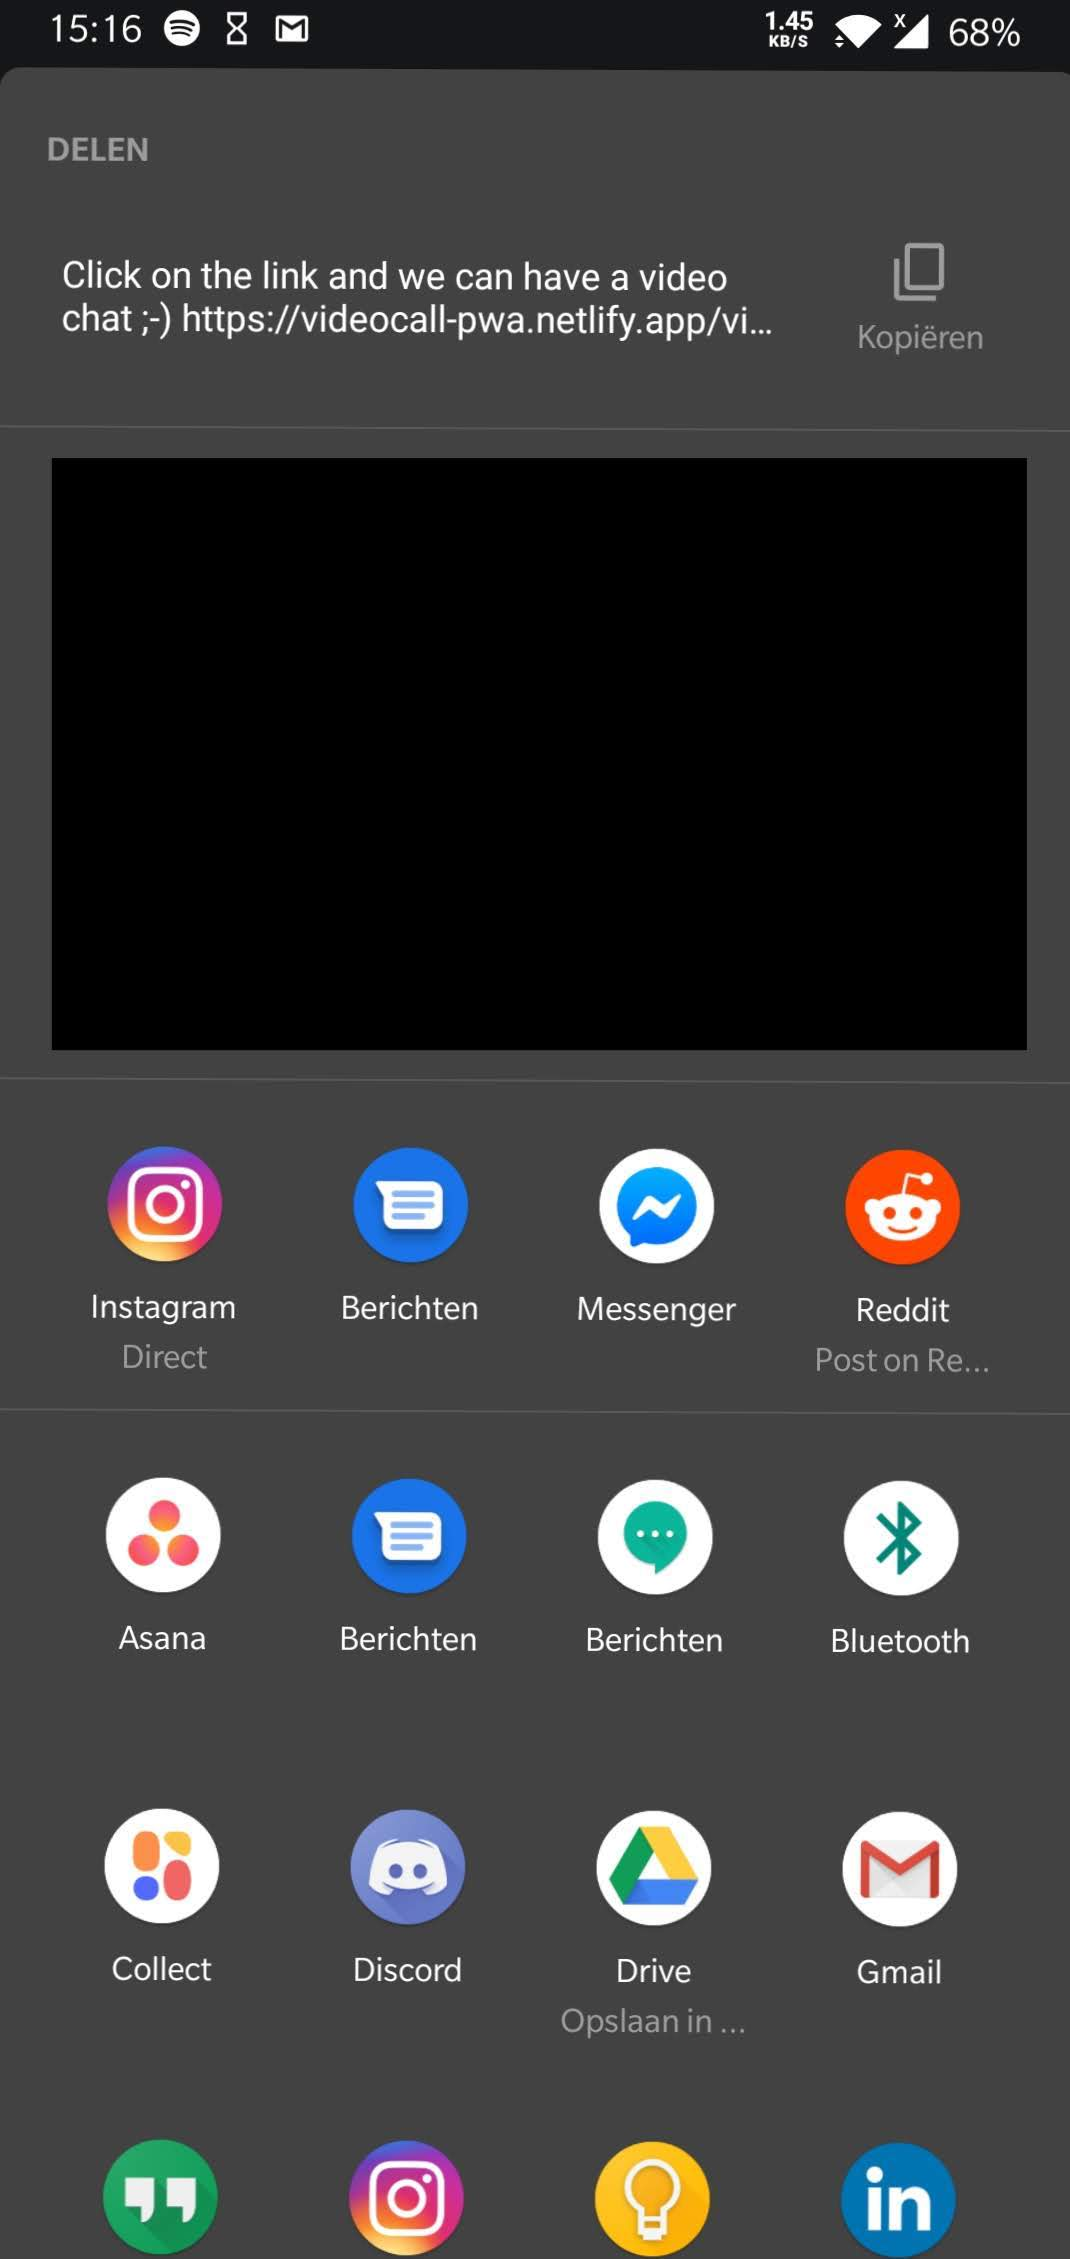
\includegraphics[width=35mm]{./img/share-android.jpg}{}
			\caption{native share-menu op Android}
			\label{fig:shareChrome}
		\end{figure}

		Als de gebruiker een browser gebruikt die deze functie niet ondersteunt, zal de clipboard API gebruikt worden.
	
		De clipboard API kan gebruikt worden om items in het klembord van de gebruiker te plaatsen of om het klembord uit te lezen.
		
		Deze web-API werd gebruikt om eenvoudig de link van de 'room' te kunnen delen met een persoon die gecontacteerd zal worden.
		
		Volgende code zal de link genereren die de uitgenodigde persoon kan gebruiken. Deze link zal in het klembord van de gebruiker geplaatst worden.
		
		De eerste keer dat dit proces uitgevoerd wordt, zal de gebruiker expliciet toestemming moeten geven om het klembord te mogen gebruiken.

\begin{lstlisting}
navigator.clipboard
  .writeText(`http://localhost:3000/visitroom/${roomownername}/${roomname}`)
  .then(() => {
    alert("coppied!! share the coppied link with somebody");
  });
};
\end{lstlisting}

		\subsubsection{Progressive enhancement}

			Bij deze feature werd er progressive enhancement toegepast. 
			In het beste geval wordt het native deelmenu getoond. Als dit niet beschikbaar is, zal de link gekopieerd worden in het klembord.
			Als ook dit niet beschikbaar is, of de gebruiker heeft geen toestemming gegeven, zal er een boodschap getoond worden waar de gebruiker de link zelf kan kopiëren en delen.
		
\begin{lstlisting}
if('share' in navigator){jesu
	// ... code voor het delen via een native menu ...
}
else{
	//... code voor het kopiëren van de link ...
	.catch(() => {
		//tonen van een boodscahp met de link die gedeeld moet worden
		swal(`you can share this link:
			https://videocall-pwa.netlify.app/visitroom/${owner}/${room}
		`);
	});
}
\end{lstlisting}


	\subsection{Push notificaties}
	
		Een van de grote voordelen van een PWA ten opzichte van een traditionele website is dat het push notificaties kan sturen naar de gebruiker.
		
		Er wordt aangeraden om de 'web-push' library te gebruiken om push notificaties te implementeren.
		
		In deze applicatie worden push notificaties gebruikt in twee use-cases:
		\begin{itemize}
			\item 	Als een bezoeker in een 'room' komt, zal de eigenaar van die 'room' een melding krijgen. Een voorbeeld van deze melding is te zien in figuur \ref{fig:notificationMacOS}.
			\item 	De administrator van de applicatie kan een notificatie naar alle gebruikers versturen vanuit een admin scherm.
		\end{itemize}	
		
		\paragraph{Abonneren op push notificaties}
			 De gebruiker moet expliciet toegang geven aan de webapplicatie om push notificaties te mogen gebruiken.
			 
\begin{lstlisting}
const sw = await navigator.serviceWorker.ready;
let pushSub = await sw.pushManager.subscribe({
      userVisibleOnly: true,
      applicationServerKey: 'public VAPID key'
})
\end{lstlisting}

			Dit stukje code zal een subscription teruggeven dat opgeslagen moet worden in de databank bij de gebruiker. Deze subscription is uniek voor de gebruiker, de browser en het toestel.
			\autocite{Gaunt2019a}
	
\newpage
			Voorbeeld van een subscription:
	
\begin{lstlisting}
{
   "endpoint":"https://fcm.googleapis.com/fcm/send/fOkirMCCHhM:..."
   "expirationTime":null,
   "keys":{
      "p256dh":"BBwYLrPvd2IIAo4cWsJhXRD2g9aFyL1Q3K9cuWh_...",
      "auth":"0orvSHRZrMb3zP0yIpUAcg"
   }
}
\end{lstlisting}


		\paragraph{Backend}
			De backend moet in een eerste fase gebruikt worden om de VAPID keys te genereren.
			
			Vapid keys of application server keys zijn uniek voor de server.
			
			Deze vapid keys zorgen ervoor dat de push services van de verschillende browsers weten van welke applicatie de notificaties afkomstig zijn. Hierdoor kan het ook de applicatie beveiligen en enkel deze server toestaan notificaties te sturen naar de applicatie.
			
			Elke browser heeft zijn eigen push service waar een applicatie server aan kan vragen om een notificatie te sturen naar een bepaald toestel.
			\autocite{Gaunt2020}
			
			Deze vapid keys kunnen in de applicatie server gegenereerd worden aan de hand van volgende code:
			
\begin{lstlisting}
console.log(push.generateVAPIDKeys)
\end{lstlisting}

			Dit zal een publieke en een private sleutel weergeven in de console. Deze moeten dan op een veilige plaats opgeslagen worden.
			
			Eens de server de Vapid keys heeft, kan deze een notificatie verzenden.
			
\begin{lstlisting}
push.setVapidDetails(
    "mailto:mai",
    secrets.vapIdKeys.publicKey,
    secrets.vapIdKeys.privateKey
  );
  
 push.sendNotification( sub,  JSON.stringify({payload})
\end{lstlisting}

			Er moet ook een geldig e-mailadres opgegeven worden. Dit e-mailadres zal gebruikt worden door de push service als er problemen zijn met jouw applicatie.
			
			De push notificatie kan dan verzonden worden met eventueel extra informatie in de payload.
			
		\paragraph{Service worker}
		
			Op basis van de subscription die in de backend werd verzonden, zal de service worker van de juiste gebruiker geactiveerd worden.
			
			De service worker zal aan de hand van een 'eventListener' geactiveerd worden en een notificatie tonen op het toestel.
			
			
\begin{lstlisting}
self.addEventListener("push", function (e) {
	//handle notification
}
\end{lstlisting}
			
			Als de backend extra informatie heeft meegegeven, dan kan deze uitgelezen worden.
\begin{lstlisting}
  const payload = JSON.parse(e.data.text())
\end{lstlisting}
			
			Vervolgens kan er een notificatie gevormd worden zoals eerder toegelicht in hoofdstuk~\ref{ch: Wat is een PWA} van deze scriptie.
			
\begin{lstlisting}
options = {
      body: "Open the app and say hi!",
      icon: "images/example.png",
      vibrate: [300, 50, 100],
      data: {
        dateOfArrival: Date.now(),
        primaryKey: "2",
      },
    };

    e.waitUntil( self.registration.showNotification(`notification title`, options)
\end{lstlisting}

	\begin{figure}[H]
		\centering
		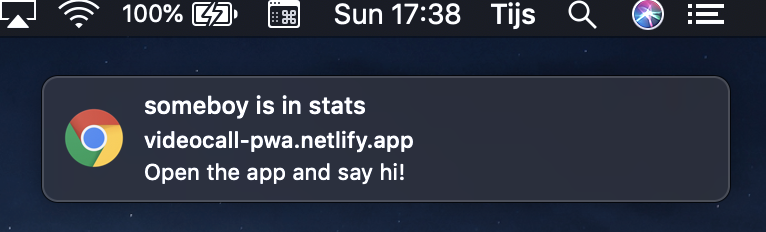
\includegraphics[width=80mm]{./img/notificationMacOs}{}		
		\caption{notificatie op macOS}
		\label{fig:notificationMacOS}
	\end{figure}
			
	\subsection{Local storage}
		
		Om een ervaring aan te bieden zoals op native applicaties is het belangrijk om de gebruiker aangemeld te houden tussen sessies.
		
		Als een gebruiker zich aanmeldt, wordt deze opgeslagen in de local storage.
		
		Zolang de gebruiker de local storage niet manueel verwijdert, zal dit blijven bestaan. 
		\autocite{Mozilla2020d}
		
	\subsection{Web RTC}
		
		Web RTC is een verzameling van Web API's die real time communicatie  op het web mogelijk maken. 
		
		In deze applicatie werd Web RTC gebruikt om:
		\begin{itemize}
			\item de camera van het toestel te gebruiken en een video-stream op het scherm te tonen
			\item een peer-to-peer connectie op te zetten tussen twee gebruikers
			\item video tussen beide gebuikers te streamen
		\end{itemize} 
		\autocite{webRTC2020}
		
		Web RTC maakt gebruik van een peer-to-peer connectie tussen de twee gebruikers. Tijdens het bellen is er dus geen server nodig. Echter, er is wel een server nodig om de connectie tussen beide tot stand te brengen.
		
		\paragraph{Video-stream}
			De video-stream zal verkregen worden via het navigator object. Bij het opvragen van een video-stream zal de browser automatisch toestemming vragen aan de gebruiker of de camera en de microfoon gebruikt mogen worden.
			
			Als de applicatie toestemming gekregen heeft, wordt er een video-stream verkregen.
			Deze stream zal opgeslagen worden in de state van de applicatie en zal in een HTML5 video element geplaatst worden.
		
\begin{lstlisting}
navigator.mediaDevices.getUserMedia({ 
		video: true,
		audio: true 
	}).then((stream) => {
		setYourVideoStream(stream);
		if (yourVideo.current) {
			yourVideo.current.srcObject = stream;
		}
	});
\end{lstlisting}


		\paragraph{Peer-to-peer verbinding met streaming}
			Bij deze applicatie werd \href{https://github.com/feross/simple-peer}{simple-peer} gebruikt. Dit is een abstractie van webRTC die het opzetten van peer-to-peer verbindingen eenvoudiger maakt.
			
			Voor beide gebruikers zal er een peer object aangemaakt worden.

\begin{lstlisting}
const peer = new Peer({
	initiator: true,

	stream: yourVideoStream,
});
\end{lstlisting}
			
			Vervolgens zullen er listeners toegevoegd worden aan deze objecten die geactiveerd worden op basis van het andere peer-object.
			
\begin{lstlisting}
peer.on("signal", (data) => {
	// code wordt uitgevoerd als er een andere peer aangemaakt wordt
});

peer.on("stream", (stream) => {
	// code wordt uitgevoerd als de andere peer start met het streamen van een video
});
\end{lstlisting}

		\paragraph{Performantie}
		
			De performantie van de applicatie werd gemeten aan de hand van de statistieken van de video-elementen waarin de stream getoond wordt. Bij beide tests was een MacBook Pro de administrator van de meeting en werd een Oneplus6 toegevoegd aan het gesprek als gast. De statistieken werden gemeten op het toestel van de administrator.
			
			\begin{table}[H]
			\centering
			\begin{tabular}{lll}													& Zoom 			& PWA \\
				gemiddeld aantal frames per seconde van ontvangende video 	 & 14				&  34 \\
				gemiddeld aantal frames per seconde van verzonden video		   & 26				   & 30	 \\
				resolutie ontvangen video  						  & 480x640 	&  480x640  \\
				resolutie verzonden video						   & 640x360	& 	640x480\\
			\end{tabular}	
			\caption{performantie-vergelijking met Zoom}
			\end{table}
	

	\subsection{Socket.io}
	
		Zoals eerder vermeld, is er een server nodig om een peer-to-peer connectie tot stand te brengen.
		
		Deze backend werd geschreven in node.js en werd gehost op \href{https://glitch.com/}{Glitch}.
		
		De library \href{https://socket.io/}{socket.io} werd gebruikt om websockets te implementeren. Websockets zorgen ervoor dat een server met de frontend kan cummuniceren zonder dat deze er expliciet om vraagt. 
		
		In traditionele applicaties krijgt de frontend enkel data als hij hier een request voor stuurt naar de backend. Bij websockets kan de backend de frontend met data voorzien in real time.
		\autocite{Mozilla2020e}
		
		Deze real-time communicatie is nodig voor het opzetten van een peer-to-peer connectie.
		
		De backend zal de frontend informeren als er een gebruiker in een 'room' komt, vervolgens kan er een peer-to-peer connectie opgezet worden.
		
		Zowel de frontend als de backend kunnen een event sturen en naar events luisteren. Op deze manier wordt er gecommuniceerd. 	
		
			
	\subsection{Masked icons}
	
		Het startscherm van Android toestellen kan in veel verschillende vormen komen. De producent van een Android toestel kan zelf een thema ontwikkelen voor het startscherm.
		
		In verschillende thema's zullen de icoontjes er anders uitzien, in sommige thema's zullen ze rond zijn, in andere vierkant met afgeronde hoeken. 
		
		Als het icoontje niet geoptimaliseerd wordt, zoals bij figuur \ref{fig:unmasked}, zal Android er steeds voor zorgen dat het icoontje volledig zichtbaar is. Indien nodig zal er een achtergrond toegevoegd worden.
		
		Door ervoor te zorgen dat alle belangrijke elementen van het icoon binnen een 'safe zone' vallen, en door een extra property toe te voegen in het app manifest kan dit opgelost worden. In figuur \ref{fig:masked} kunnen de geöptimaliseerde iconen gevonden worden.
	
		Toe te voegen aan app manifest:
\begin{lstlisting}
"purpose": "any maskable" 
\end{lstlisting}

		In deze proof of concept werden de iconen ook 'maskable' gemaakt \ref{fig:videocallMasked}

		\begin{figure}[H]
			\centering
			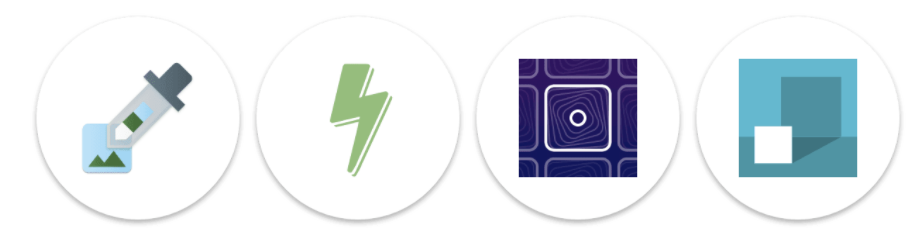
\includegraphics[width=60mm]{./img/traditionalIcons}{}
			\caption{niet-geoptimaliseerde iconen \autocite{Oakes2019}}
			\label{fig:unmasked}
		\end{figure}
		\begin{figure}[H]
			\centering
			\includegraphics[width=60mm]{./img/maskedicons}{}
			\caption{masked iconen  \autocite{Oakes2019}}
			\label{fig:masked}
		\end{figure}
		\begin{figure}[H]
			\centering
			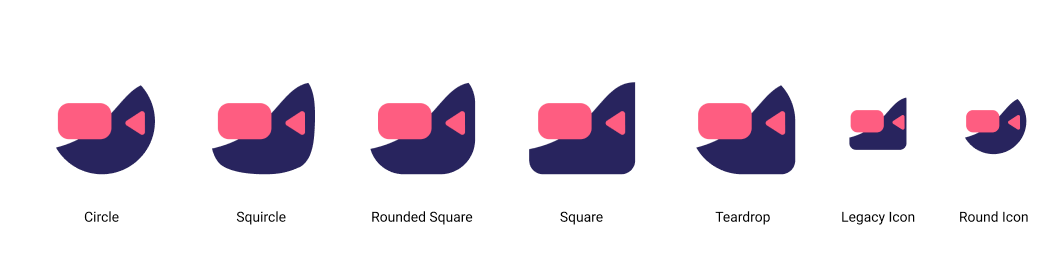
\includegraphics[width=100mm]{./img/iconPWA.png}{}
			\caption{geoptimaliseerde iconen van proof-of-concept}
			\label{fig:videocallMasked}
		\end{figure}

\newpage
\section{De applicatie}
	\subsection{Authenticatie}
		De gebruiker kan zich registreren aan de hand van een combinatie van e-mail en wachtwoord. Er is ook een optie om zich aan te melden aan de hand van Google en Facebook.
		
		
		\begin{figure}[H]
			\centering
			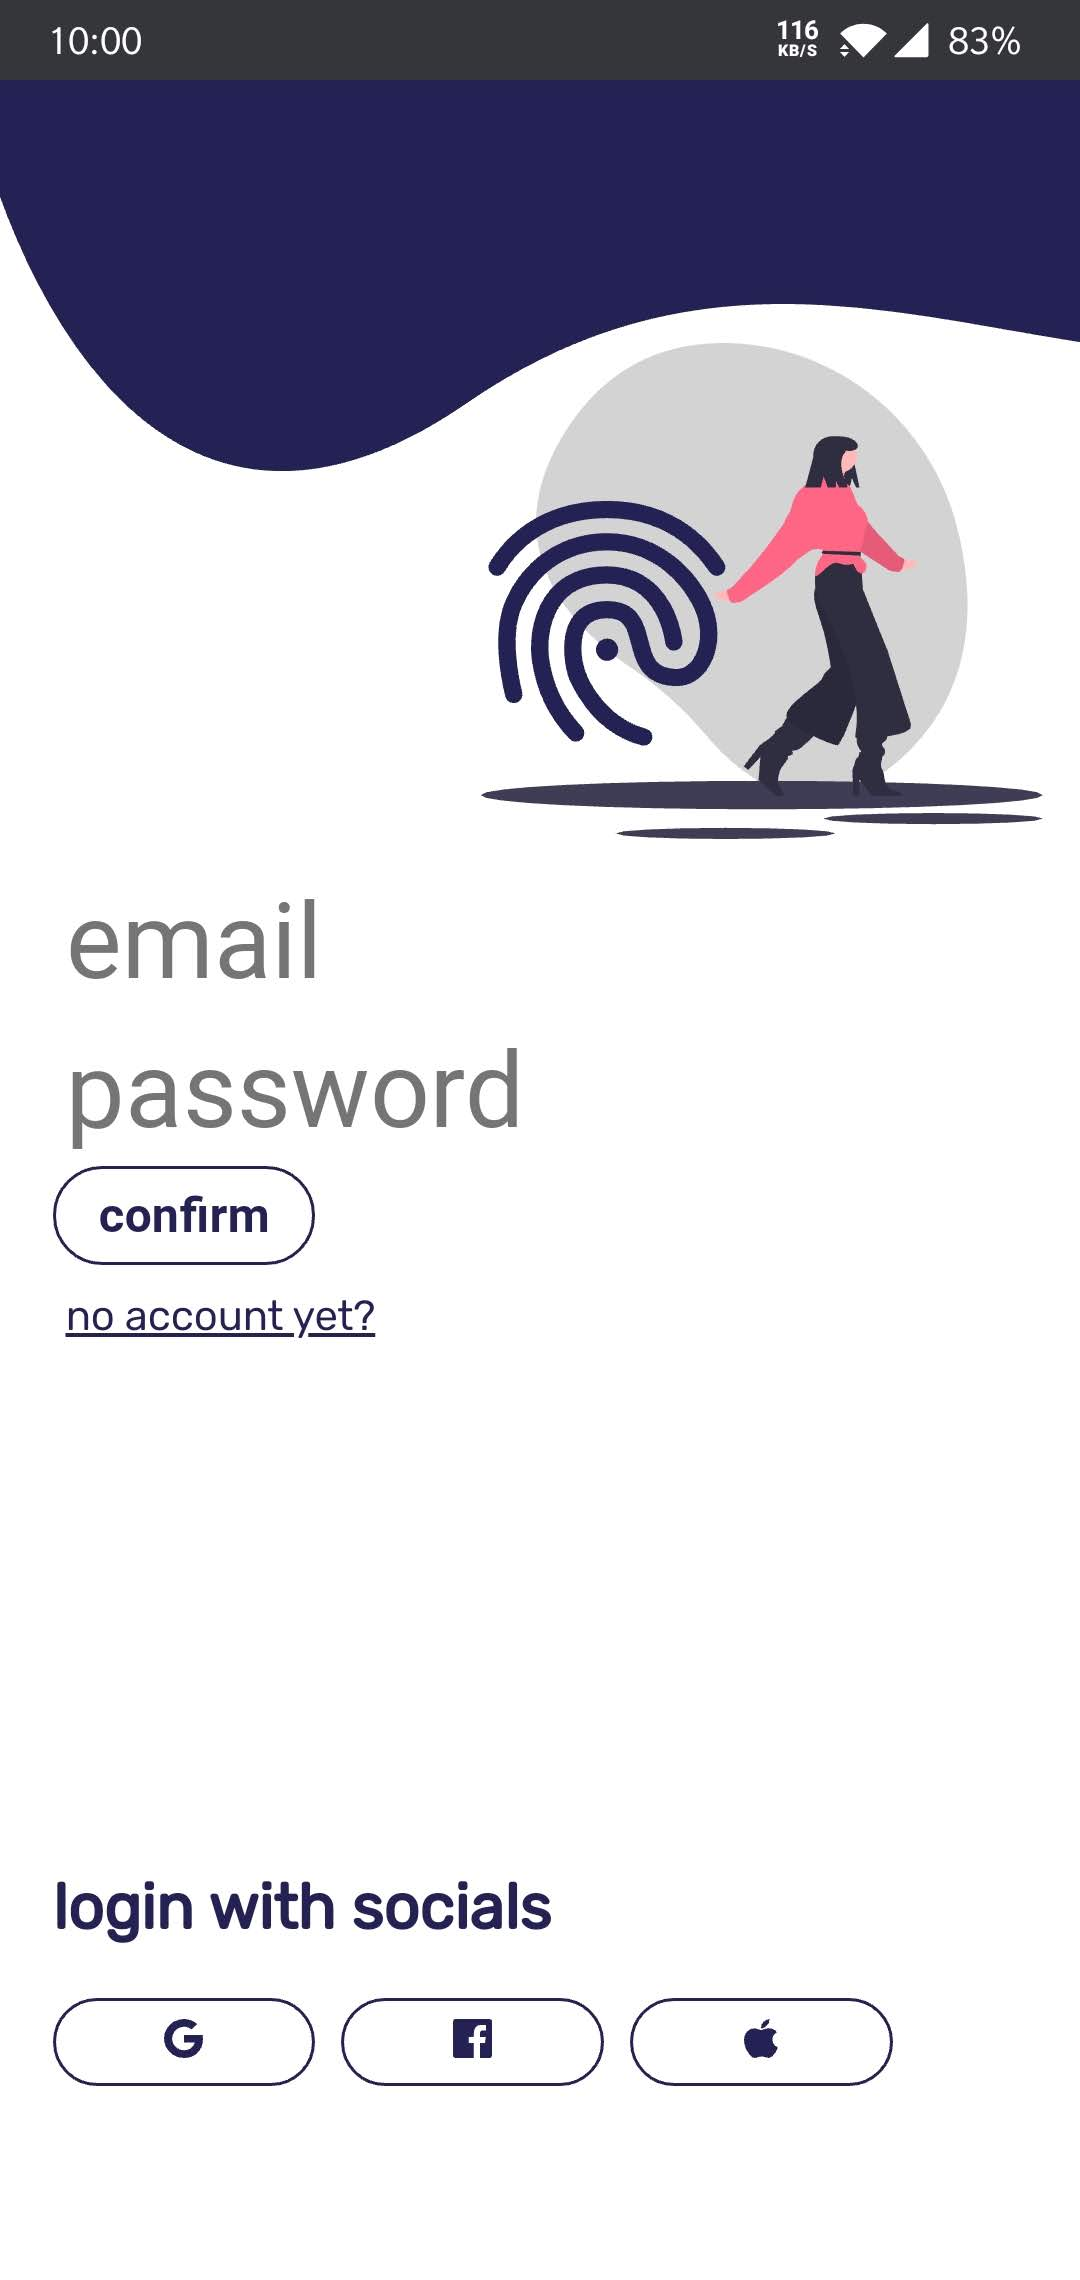
\includegraphics[width=35mm]{./img/POC/login.jpg}{}		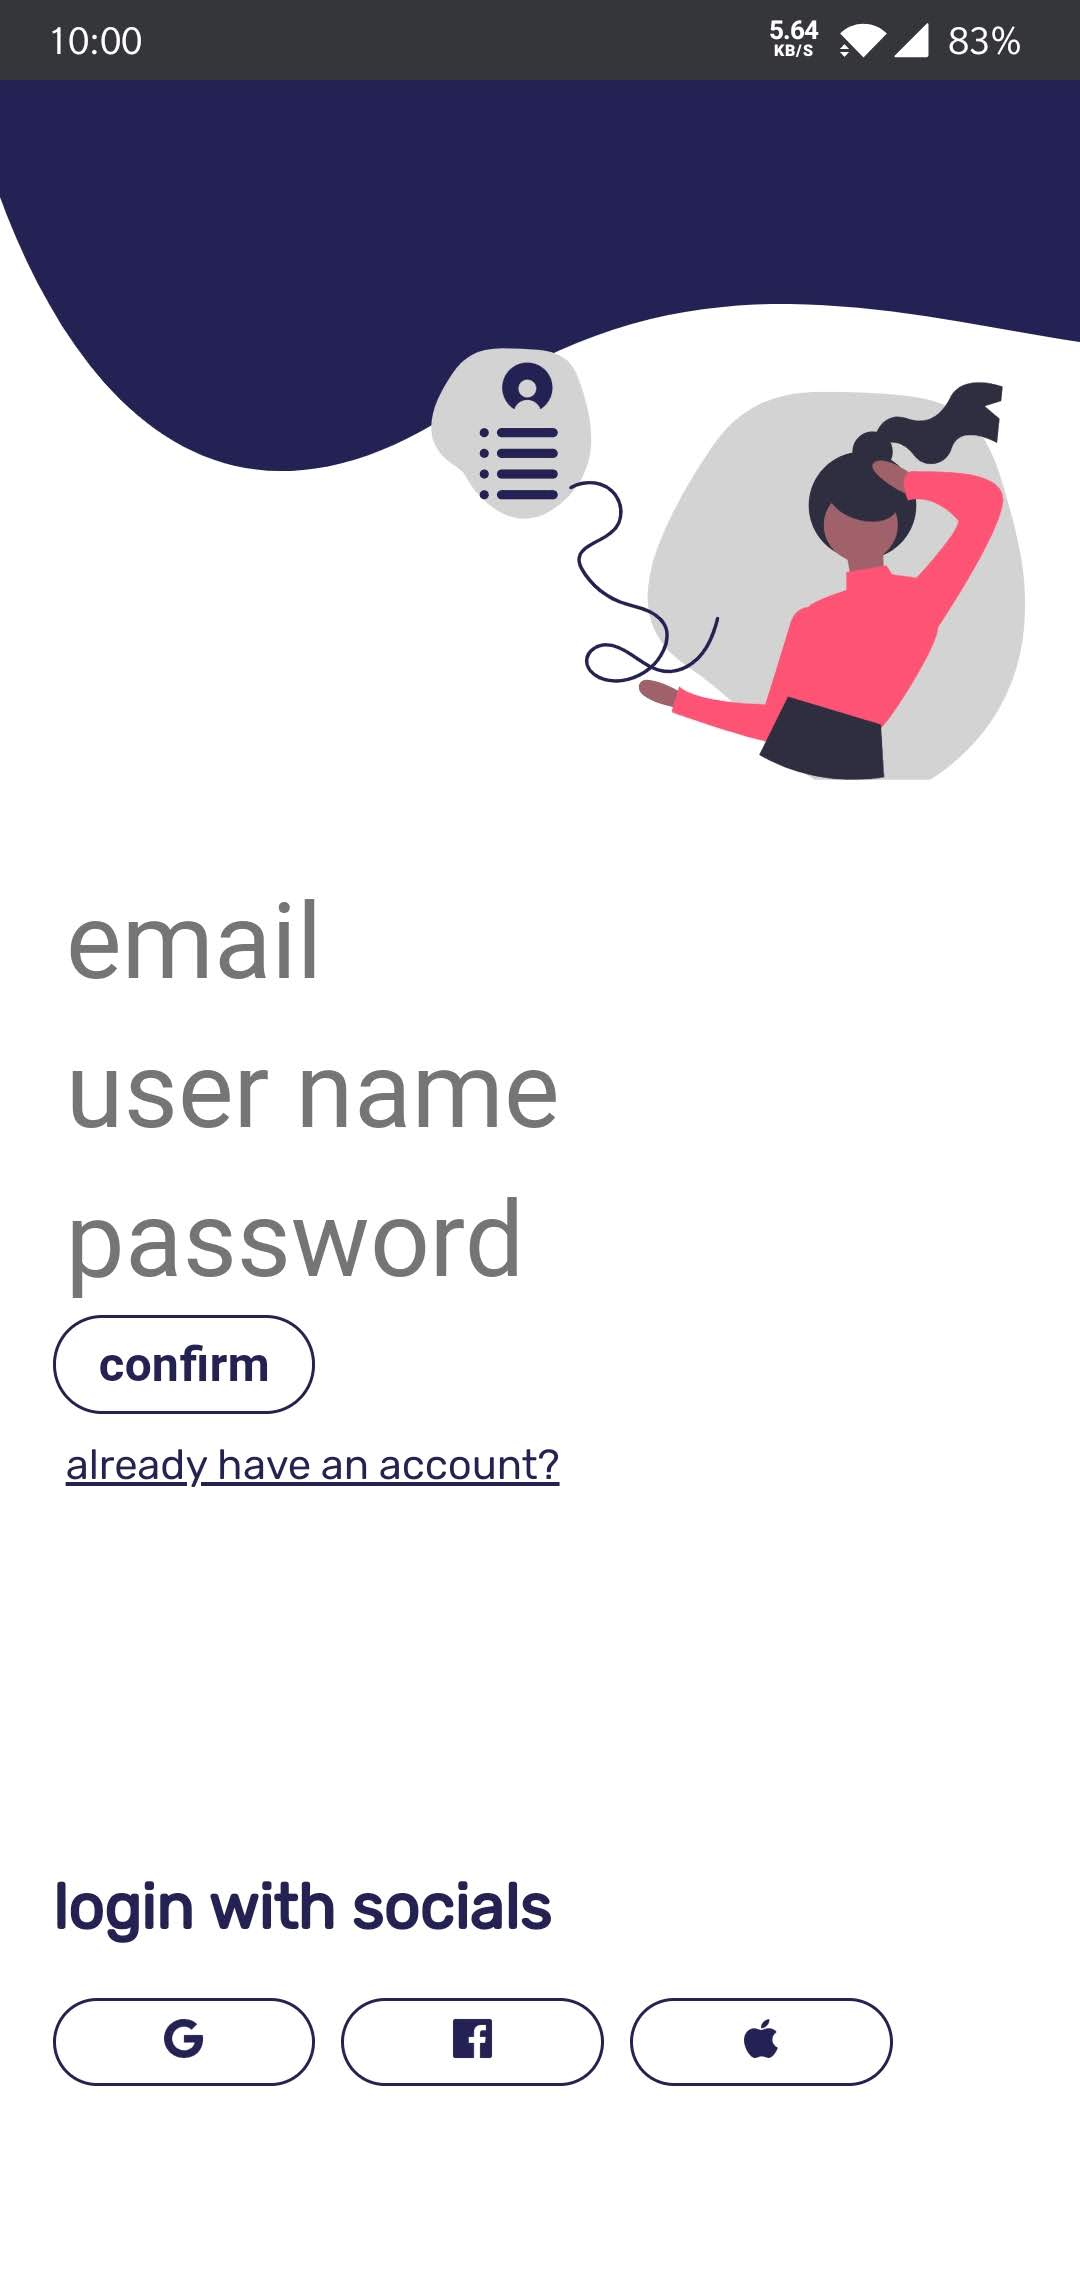
\includegraphics[width=35mm]{./img/POC/register.jpg}{}
			\caption{autenticatie-schermen}
		\end{figure}
		
		
		\newpage
	\subsection{Home}
		Dit is het scherm waar de gebruiker zal terechtkomen als hij is aangemeld. 
		Op dit scherm kan de gebruiker zijn 'rooms' beheren: hij kan nieuwe 'rooms' aanmaken, 'rooms' verwijderen en 'rooms' delen.
		
		Onderaan de pagina is er een horizontale scroll. In deze lijst heeft de gebruiker volgende opties:
		\begin{itemize}
			\item de applicatie installeren en toevoegen aan het startscherm
			\item notificaties aanzetten 
			\item afmelden
		\end{itemize}
		
			\begin{figure}[H]
				\centering
				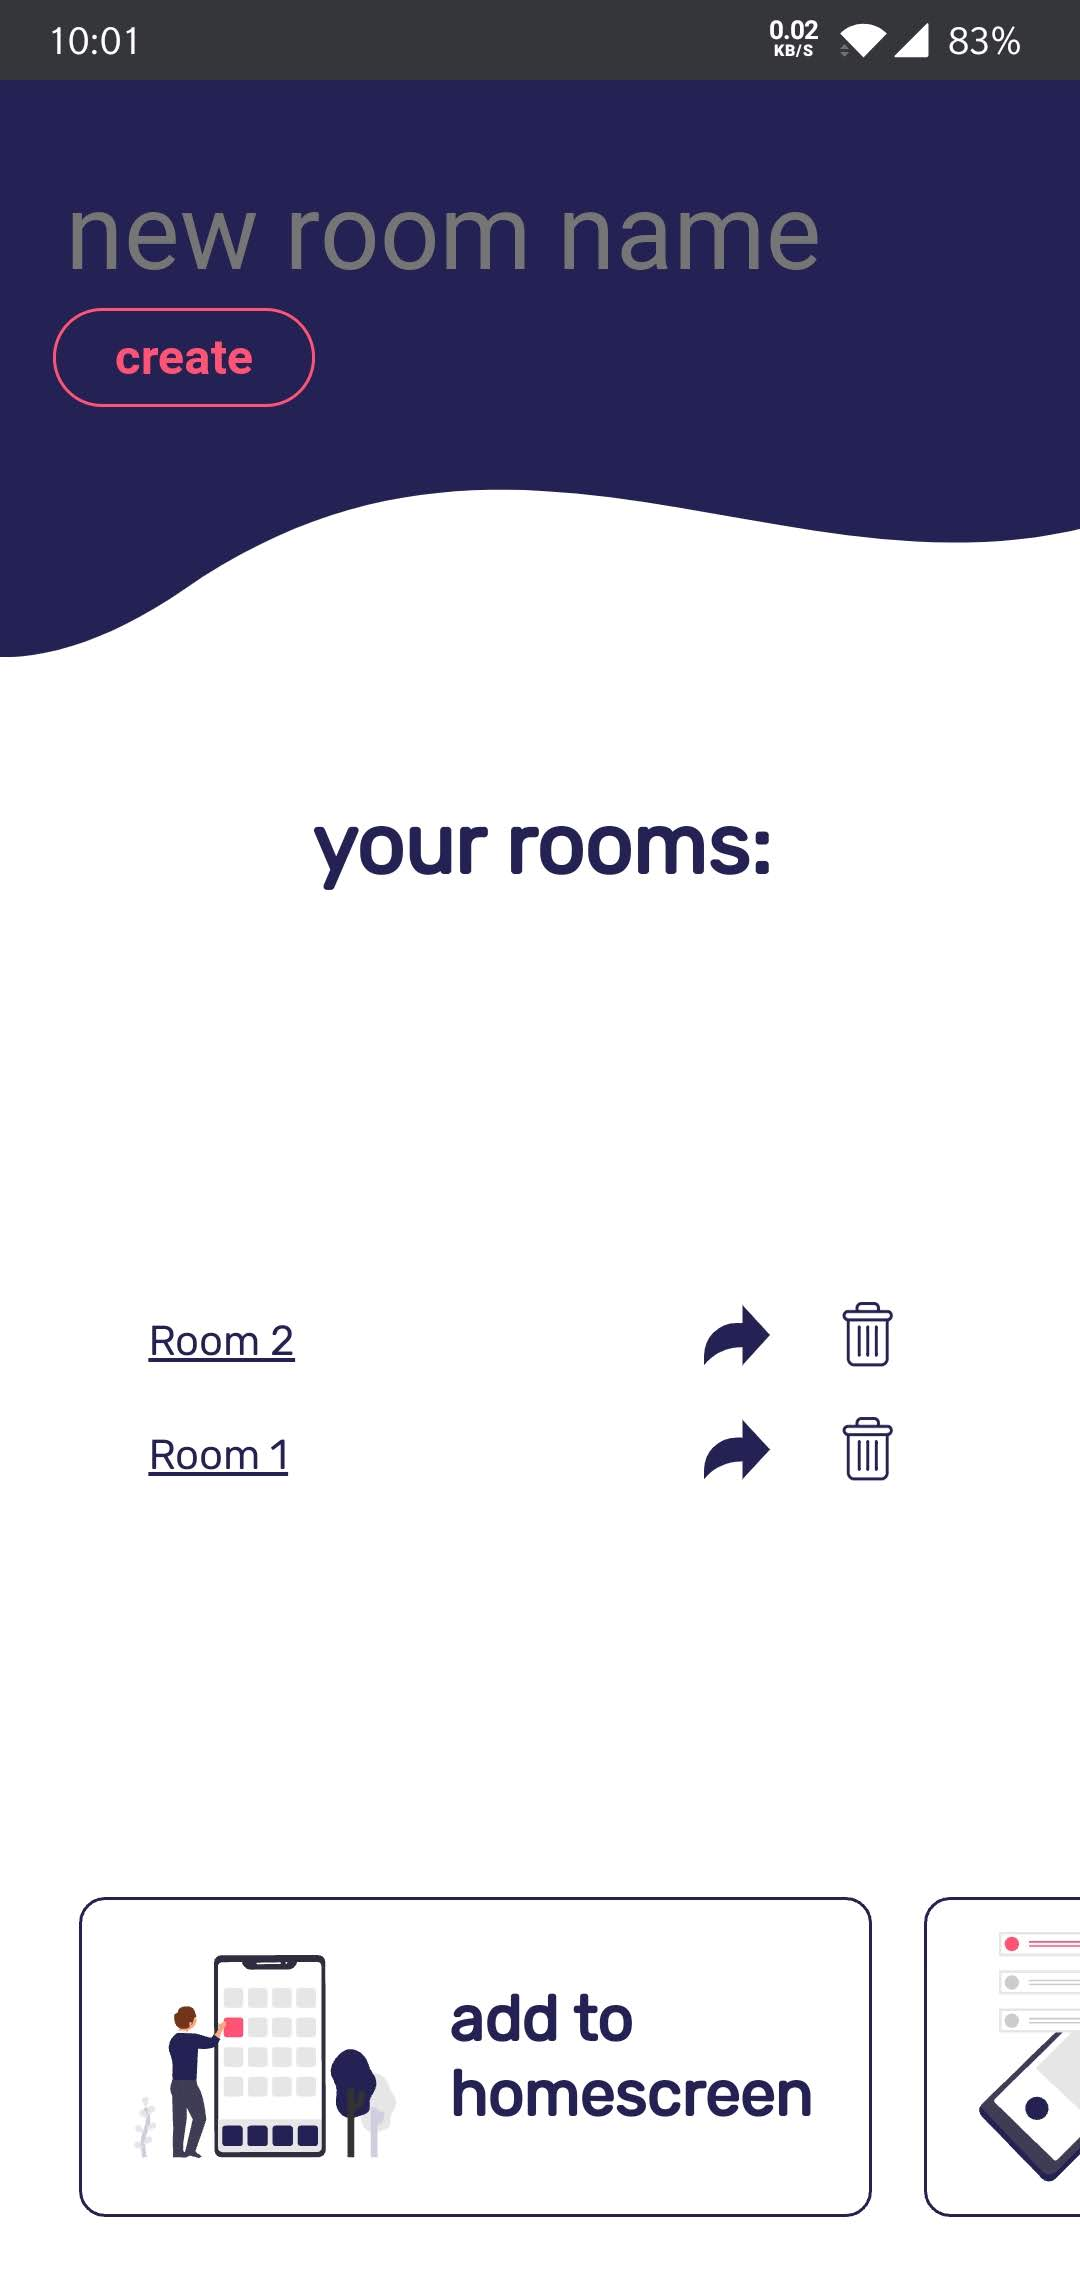
\includegraphics[width=35mm]{./img/POC/home}{}		
				\caption{homescherm}
			\end{figure}
	
	\newpage
	\subsection{Wachtschermen}
		Als er slechts één persoon aanwezig is in de 'room', zal de gebruiker op dit scherm terechtkomen. 
		
		De eigenaar van de 'room' heeft de optie om de 'room' te delen. 
		
		Als een bezoeker in de 'room' komt, zal de eigenaar een melding krijgen dat er iemand in zijn 'room' is. Door op de notificatie te klikken, gaat de eigenaar direct naar de 'room'.
						
		Als beide gebruikers aanwezig zijn, zal de bezoeker de optie krijgen om het gesprek te starten.

		\begin{figure}[H]
			\centering
			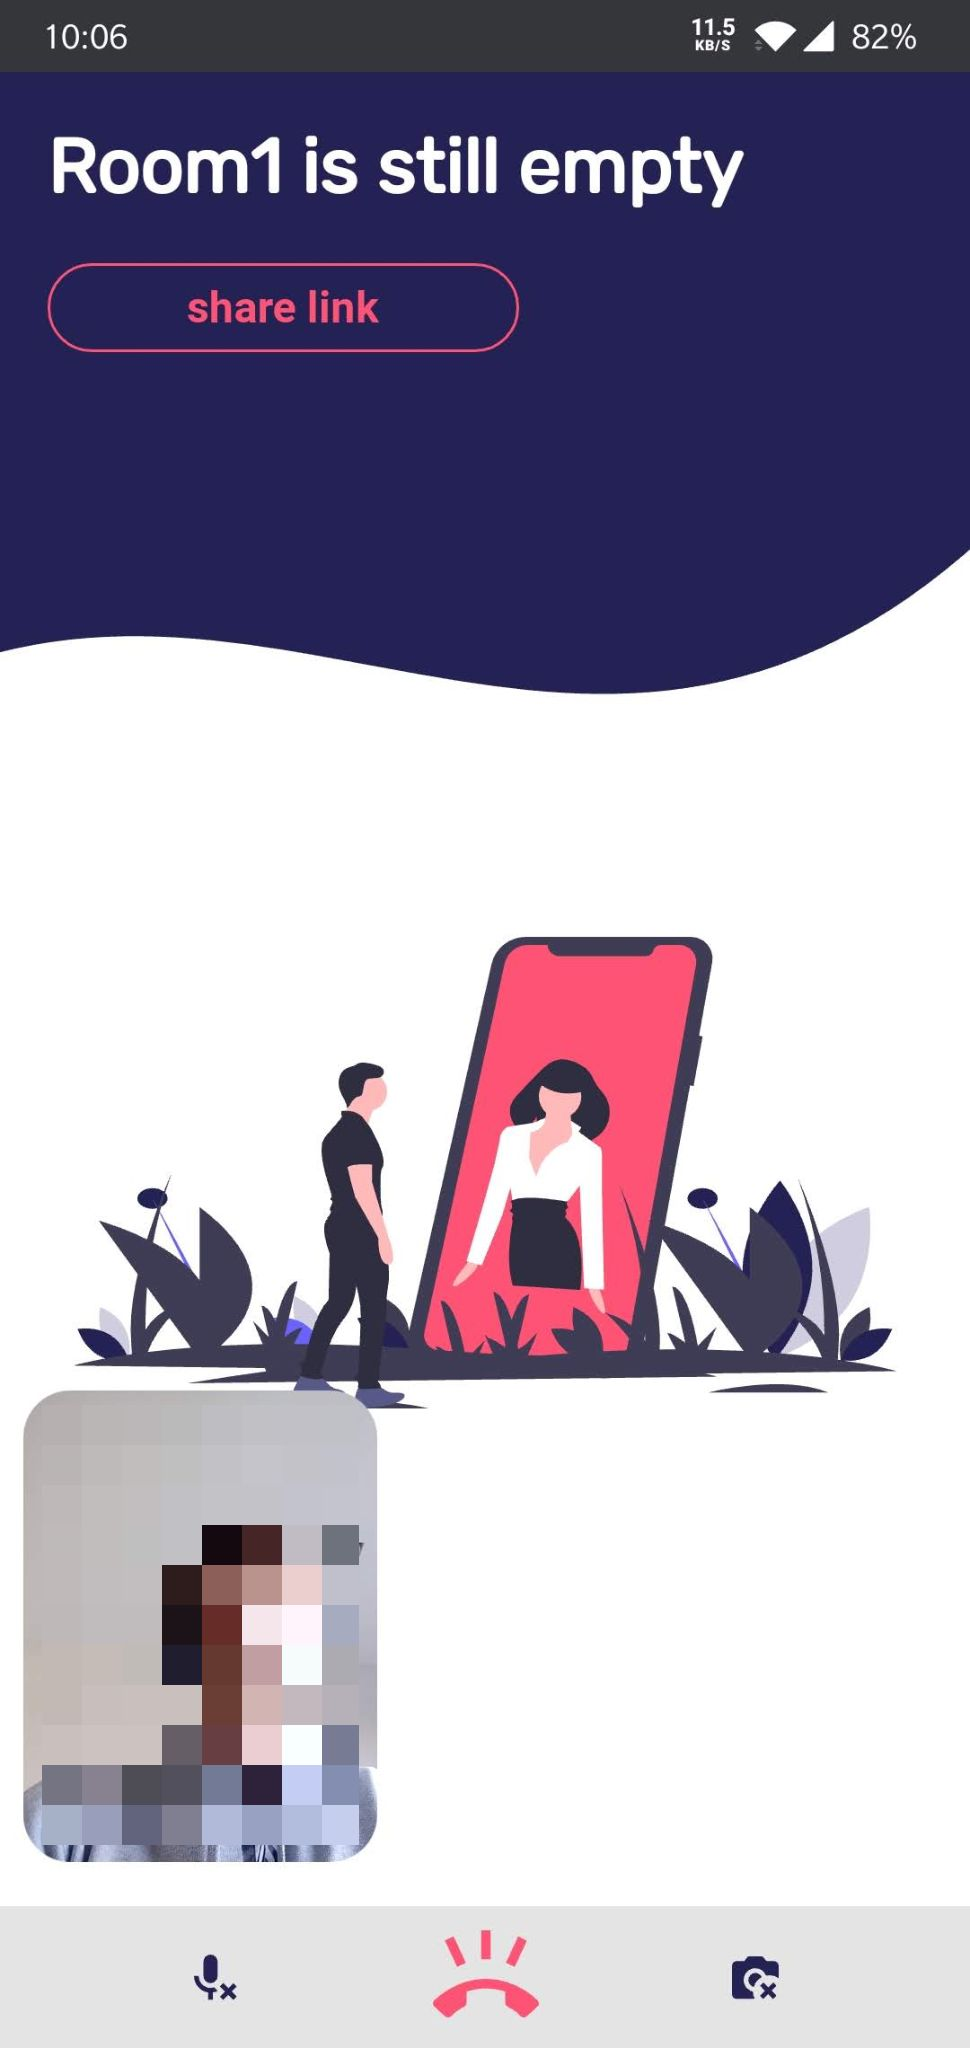
\includegraphics[width=35mm]{./img/POC/waitAsOwner.jpg}{}		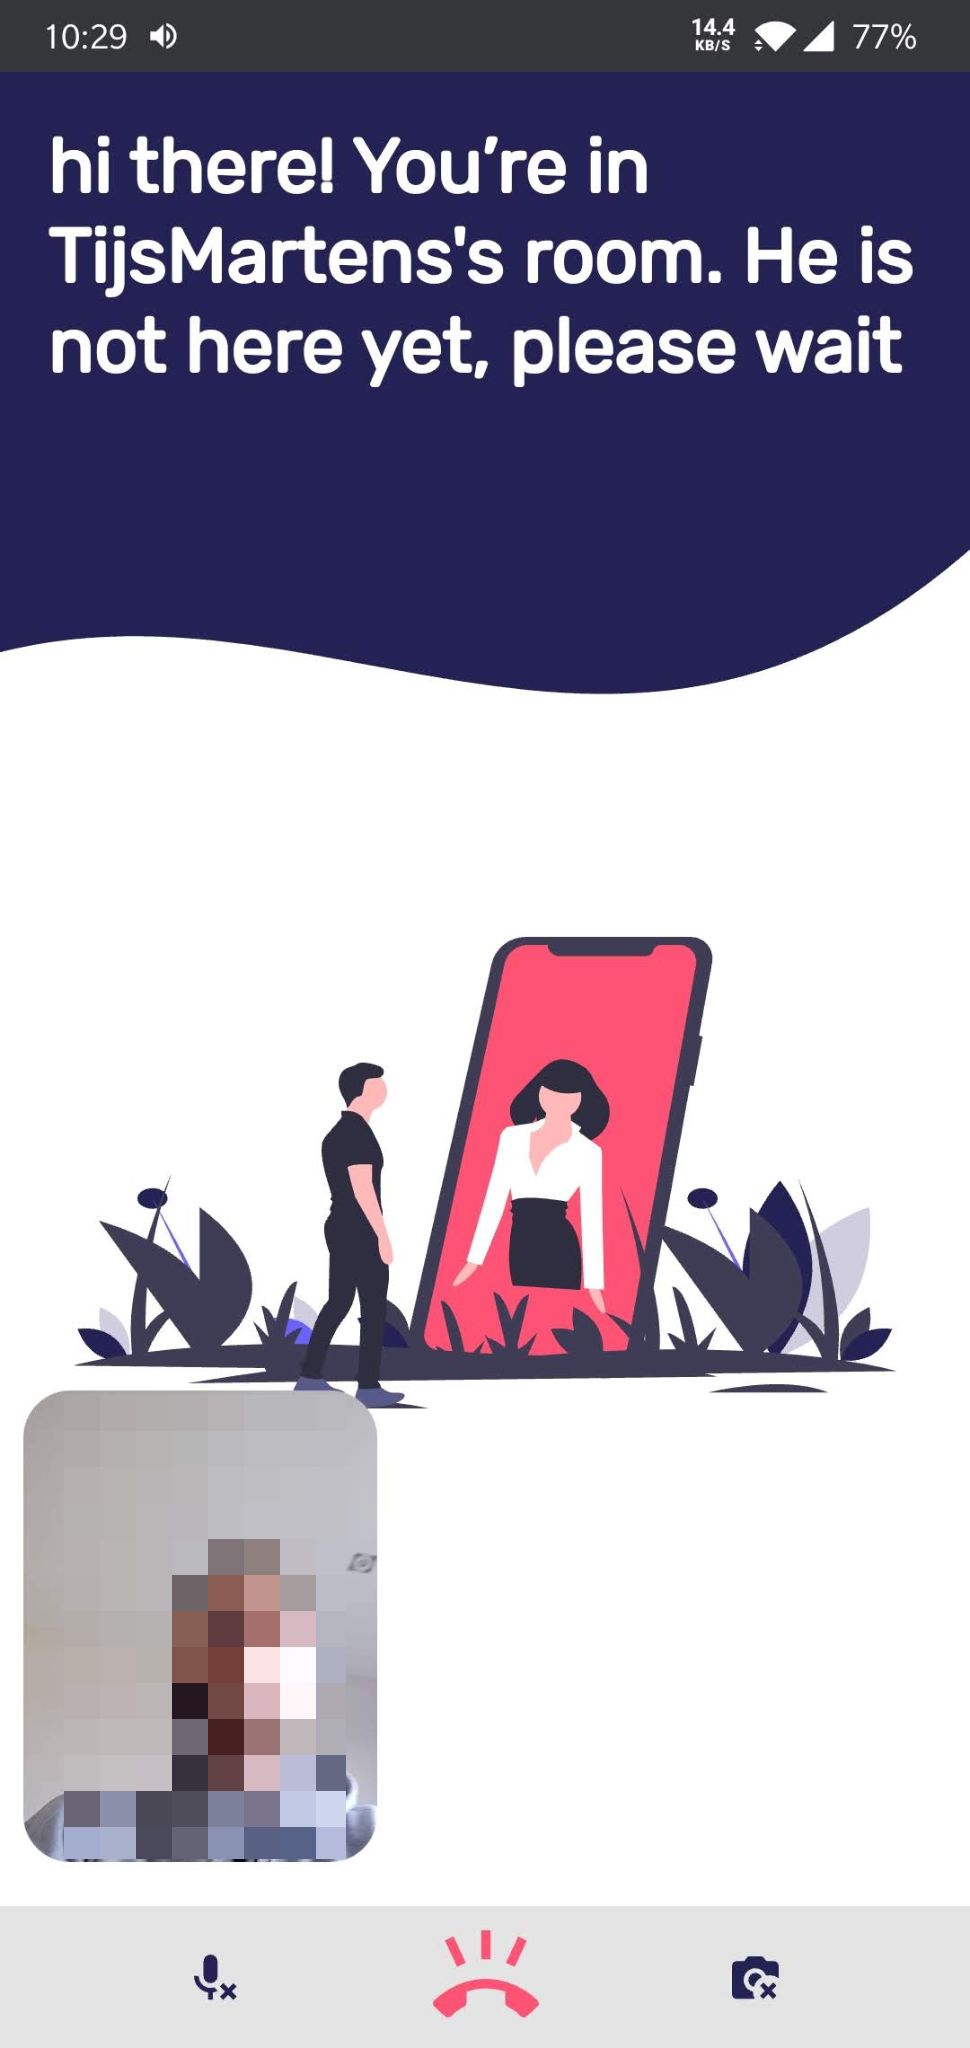
\includegraphics[width=35mm]{./img/POC/waitAsVisitor1.jpg}{}
			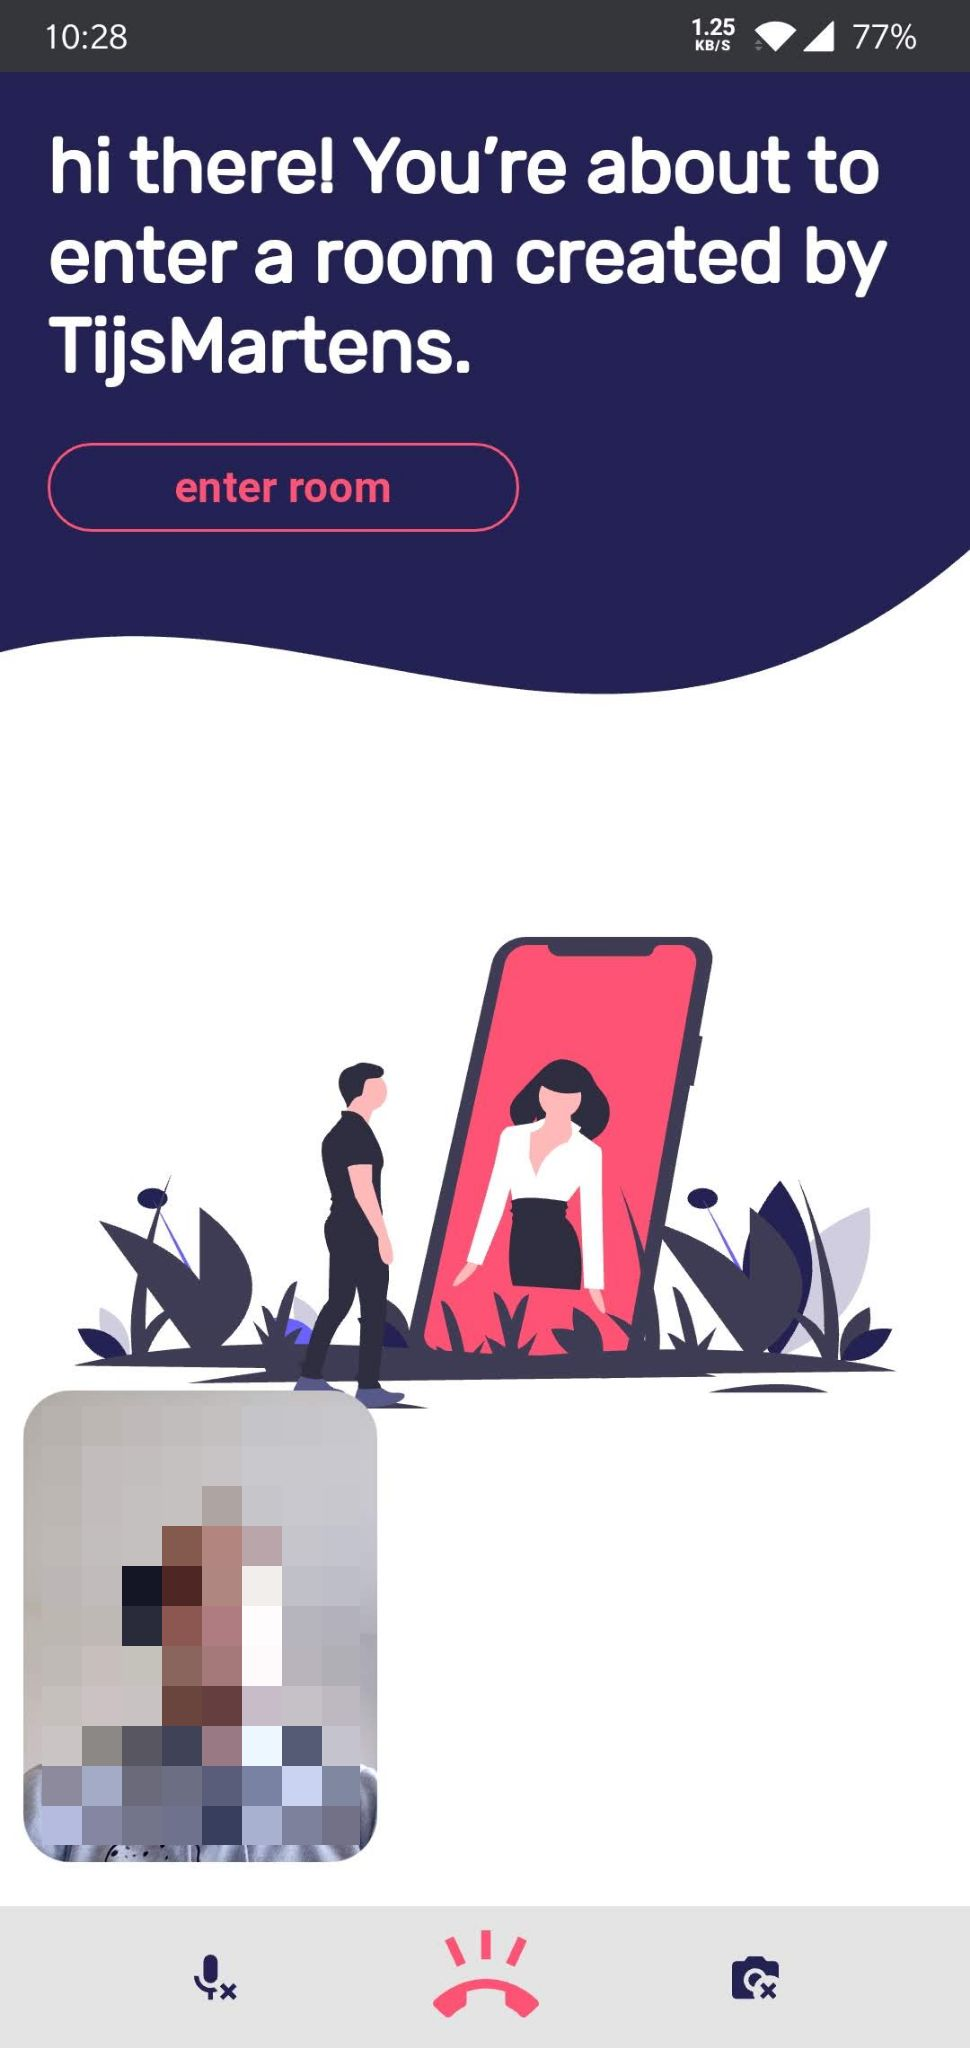
\includegraphics[width=35mm]{./img/POC/waitAsVisitor2.jpg}{}
			\caption{wachtschermen}
		\end{figure}
		
		
	\newpage
	\subsection{Room}
		In dit scherm kunnen de gebruikers een conversatie hebben. 
		
	
		\begin{figure}[H]
			\centering
			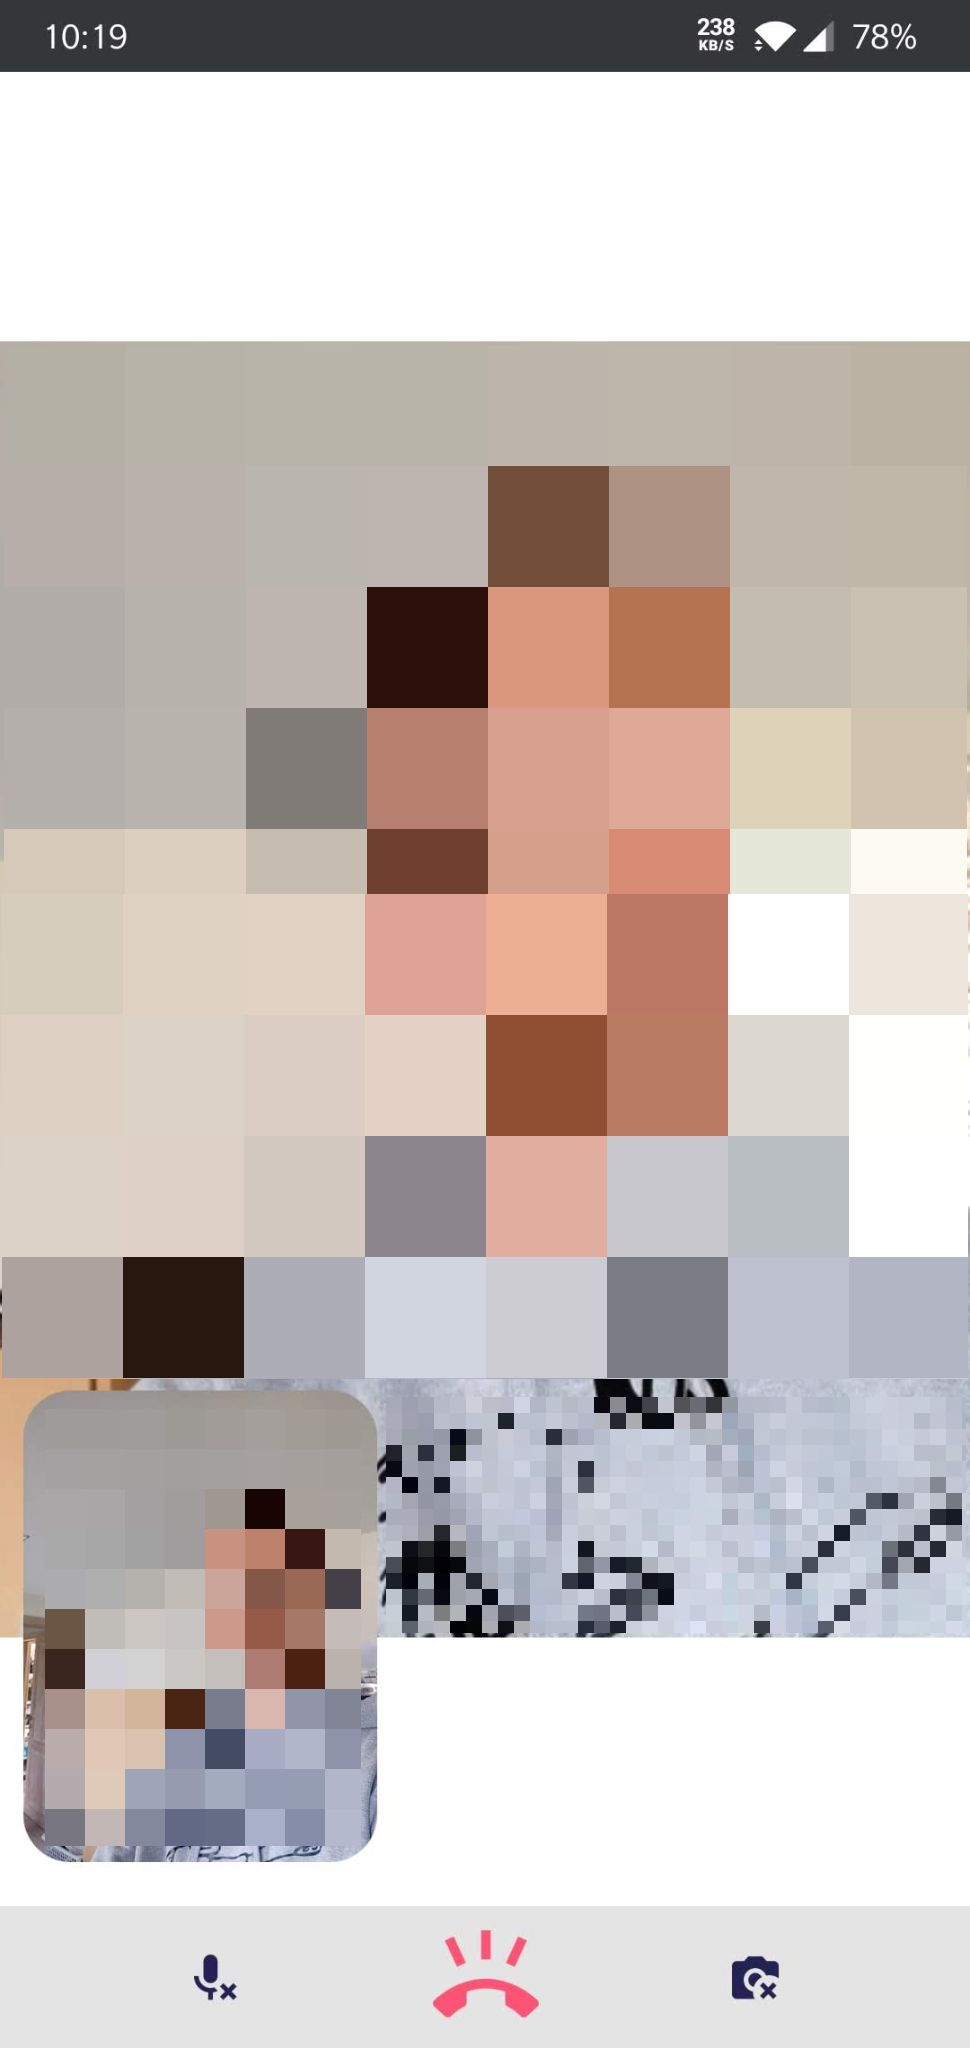
\includegraphics[width=35mm]{./img/POC/call.jpg}{}		
			\caption{belscherm}
		\end{figure}
		
	\subsection{Notificaties}
		Op dit scherm kan de administrator van de applicatie een zelf gekozen notificatie versturen naar alle gebruikers die hun goedkeuring hebben gegeven om notificaties te ontvangen.
		
		\begin{figure}[H]
			\centering
			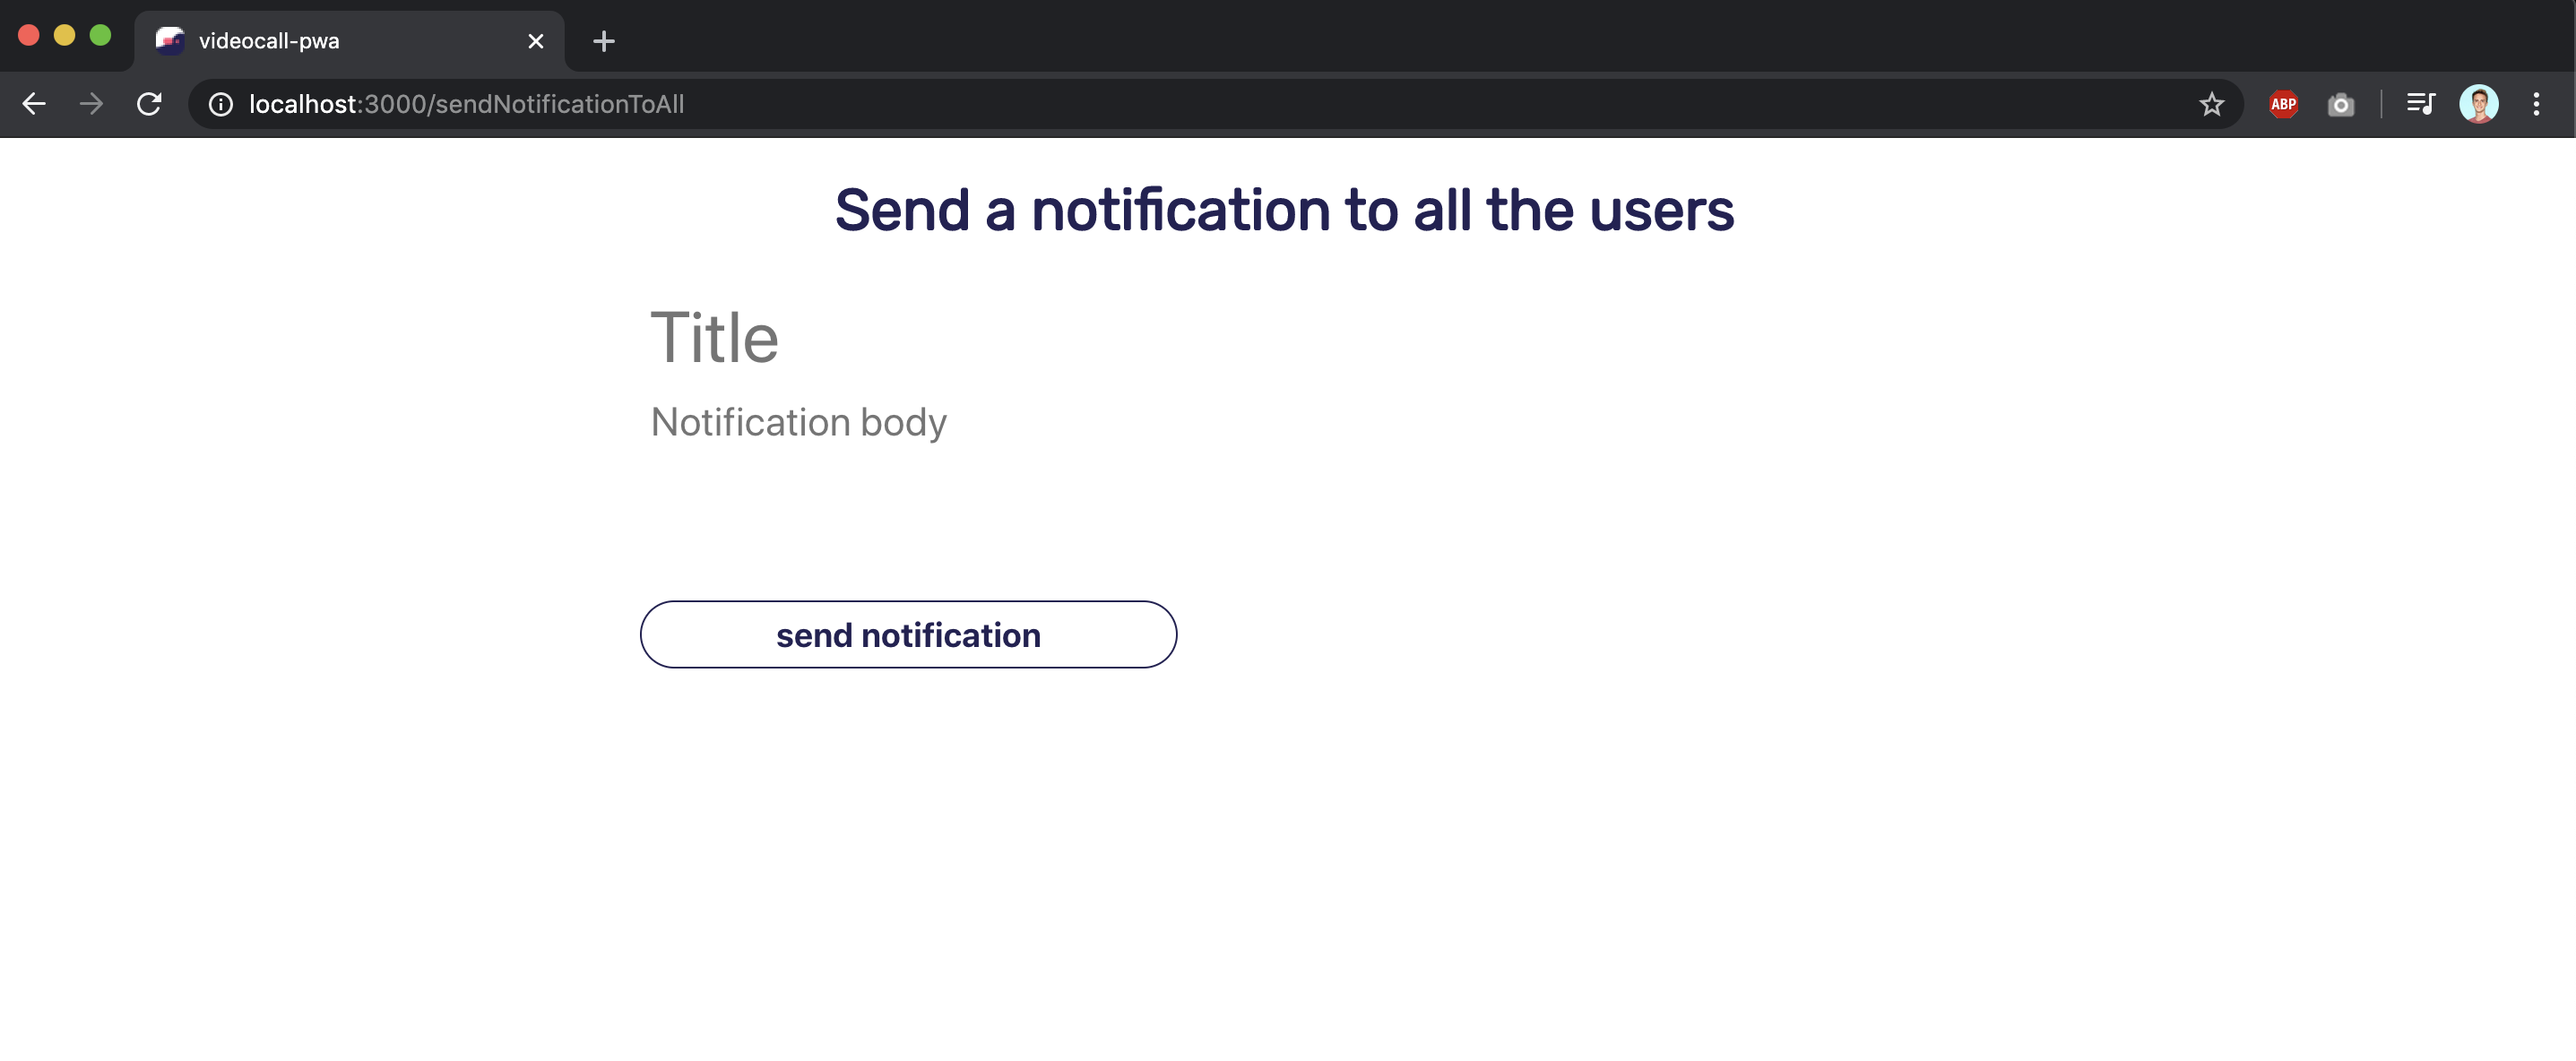
\includegraphics[width=100mm]{./img/POC/sendNoti}{}		
			\caption{scherm om manueel een notificatie te versturen}
		\end{figure}
		
\newpage
\section{Conclusie}
	
	Al de vooropgestelde requirements kunnen bereikt worden door een PWA te implementeren. 
	Native features zoals het gebruik van de camera, de microfoon, delen en notificaties konden succesvol geïmplementeerd worden in deze proof-of-concept.
	
	\subsection{Compatibiliteit en besturingssystemen}
		Zoals eerder aangehaald is één van de nadelen van PWA's de sterk variërende ondersteuning van browsers. Daarom is het belangrijk dat de applicatie ontwikkeld wordt aan de hand van progressive enhancement. 
		
		De hoofdfunctionaliteit van de applicatie moet beschikbaar zijn voor alle gebruikers. Vervolgens kan de applicatie uitgebreid worden met functionaliteiten die de ervaring verbeteren maar die niet noodzakelijk zijn.
		
		In deze applicatie is de hoofdfunctionaliteit het videobellen. Zoals aangetoond in hoofdstuk~\ref{ch: BesturingssystemenEnPWAs} wordt webRTC ondersteund op alle veelgebruikte browsers en toestellen. Er werden vervolgens extra functionaliteiten toegevoegd zoals het delen van de link via het native deel-menu, de clipboard API, push notificaties en het automatisch toevoegen aan het startscherm.
		\begin{itemize}
	  		\item Het deel-menu is enkel beschikbaar op mobiele toestellen en Safari op macOS.
	  		\item De clipboard API is beschikbaar op alle browsers en toestellen maar heeft wel de toestemming van de gebruiker nodig.
	  		\item Push notificaties hebben ook de toestemming van de gebruiker nodig en zijn beschikbaar op alle browsers en toestellen met uitzondering van:
	  				\begin{itemize}
	  			  		\item alle browsers op iOS
	  			  		\item Safari op macOS
	  		 		\end{itemize}	
  			\item Automatisch toevoegen aan het startscherm is beschikbaar op alle browsers en toestellen met uitzondering van:
	  				\begin{itemize}
	  			  		\item alle browsers op iOS
	  			  		\item Safari op macOS
	  		 		\end{itemize}	
 		\end{itemize}
 		
	\newpage		
	\subsection{Verwachting gebruiker}
		Een gebruiker die een applicatie installeert op een iOS toestel zal een andere user interface verwachten dan een gebruiker die een applicatie installeert op een Android toestel.
		
		Met een PWA kan er slechts één user interface geïmplementeerd worden. Het is dus niet mogelijk om volledig aan de verwachting van elke gebruiker te voldoen.
		
		Een gebruiker met een toestel dat op iOS werkt, is gewoon om naar de vorige pagina te navigeren door naar rechts te swipen op het toestel. Dit is een manier van navigeren die een Android gebruiker niet gewoon is. In deze proof-of-concept kan er niet met touch-gebaren genavigeerd worden. Dit kan niet 'native' aanvoelen voor de iOS gebruiker. 
		
		%todo:📈✅
		Uit de resultaten van de user-testen bleek dat veel mensen niet weten welke functionaliteit beschikbaar is voor het web. Zo wist 23,1\% niet dat een webapplicatie gebruik kan maken van de camera en 61,5\% wist niet dat een website ook offline kan werken.
		
		Dit is relevant want als een gebruiker niet weet dat een PWA dit kan doen, dan zal hij dit waarschijnlijk ook niet testen. 
		%todo: ✅resultaten van user testing - wat weet een gebruiker van het web
		
	\subsection{Gebruik van PWA's}
		%todo:✅ resultaat van user testing - zou de gebruiker PWA verkiezen boven native
		In de user-testen werd er gevraagd of een gebruiker een PWA zou verkiezen boven een native applicatie. 
		100\% van de gebruikers zou de native applicatie verkiezen boven een PWA. Het argument dat er niet geweten is dat een service ook werkt in de browser kwam meerdere keren naar boven.
		
		De testers hadden ook nog andere uiteenlopende redenen waarom ze een native applicatie verkozen:
		\begin{itemize}
	  		\item 'Heb geen reden om geen native gebruiken'
	  		\item 'Native heeft een beter gevoel'
	  		\item 'Ik vertrouw een webapplicatie minder dan een native applicatie'
	  		\item 'Ik prefereer iOS en integratie van native'
	  	\end{itemize}	
			  	
		%todo:✅ resultaat van user testing - zou de gebruiker PWA verkiezen boven native MET CONTEXT WAT PWA IS
		In het onderzoek werd vervolgens dezelfde vraag opnieuw gesteld, maar nu werd er meer info gegeven aan de testpersoon over wat PWA's zijn. De tester werd verteld dat een PWA ook op het startscherm kan staan, notificaties kan versturen, en dat de app-grootte veel kleiner is dan die van een native app. 
		%todo:📈✅
		Als deze info geweten was, zou 75\% van de gebruikers wel overwegen om een PWA te gebruiken in plaats van de native applicatie. Voor veel gebruikers was de app-grootte de overtuigende factor.
		
		Figuur \ref{fig:gebruikPWA}  toont aan dat Android gebruikers meer geneigd zijn om een PWA te gebruiken ten opzichte van iOS gebruikers.
		
		
		\begin{figure}[H]
			\centering
			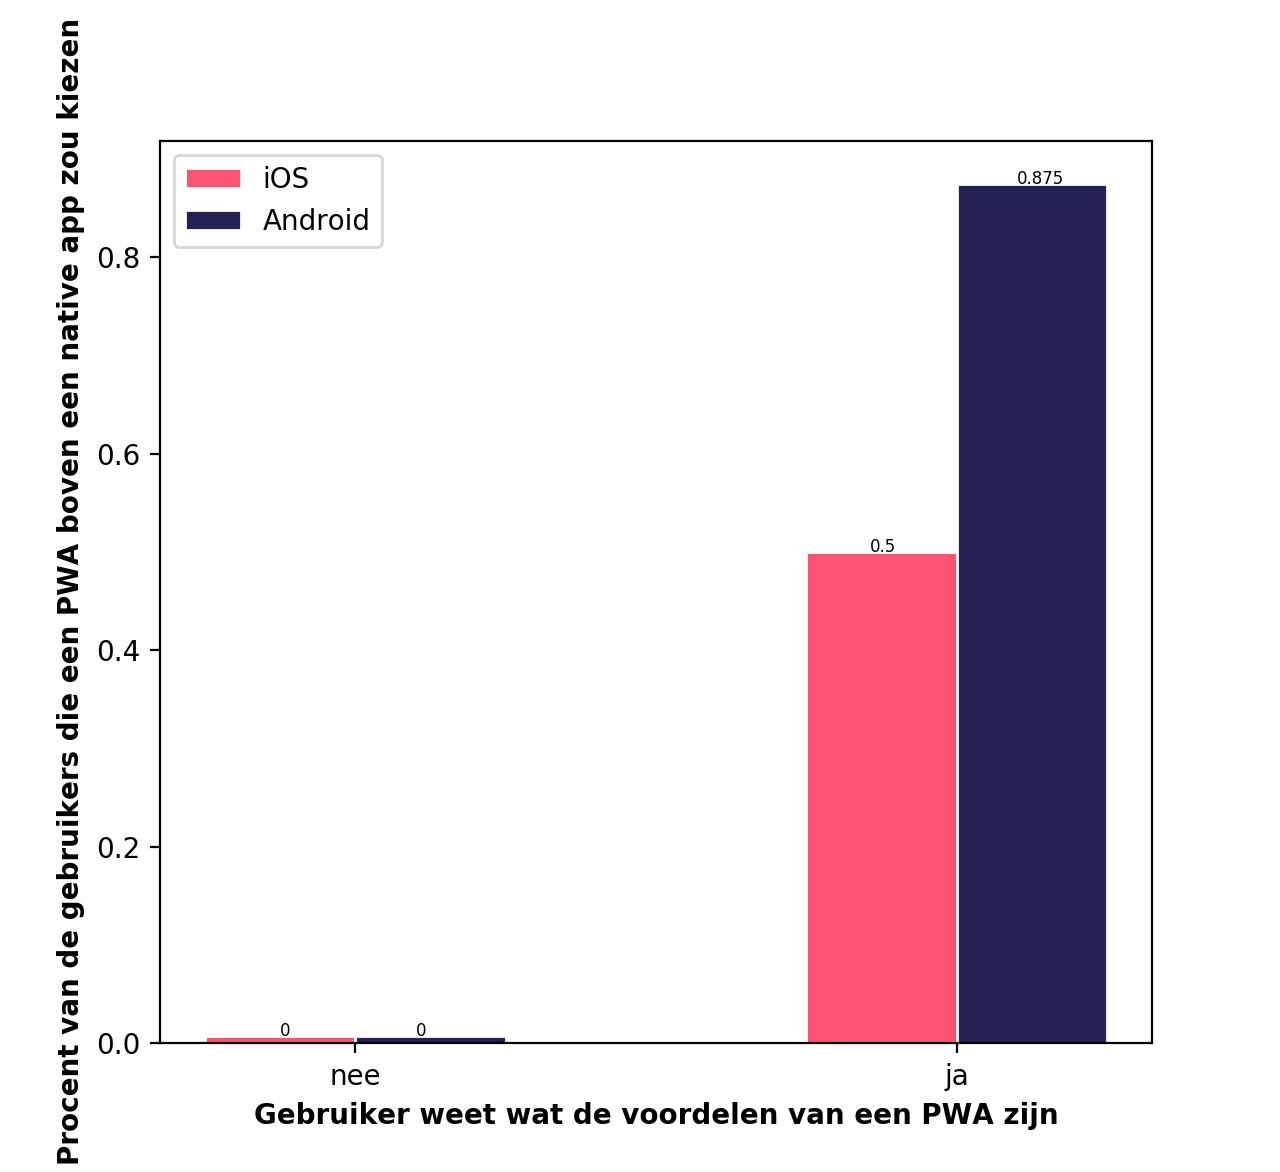
\includegraphics[width=120mm]{./img/PWA_over_Native.png}
			\caption{gebruik van PWA's}
			\label{fig:gebruikPWA}
			
		\end{figure}

		
		%todo: ✅resultaat van user testing - zou de gebruiker notificaties toestaan
		Push notificaties zijn een sterk middel om user engagement te verhogen. \autocite{Gaunt2020} Als een PWA hier gebruik wil van maken, moet de gebruiker hier expliciet toestemming voor geven. 
		
		In de tweede proof-of-concept werd deze functie geïmplementeerd. De gebruiker kan deze zelf activeren. Hij zal dus niet lastig gevallen worden met pop-up's die om toestemming vragen. Vooraleer de gebruiker de notificaties activeert, weet hij voor welke doelen dit gebruikt zal worden. Dit is volgens Matt Gaunt de beste user experience. Dit zal dan ook resulteren in een hoog aantal mensen die notificaties toestaan. \autocite{Gaunt2019c}
		
		%todo:📈✅
		Er werd aan de gebruikers gevraagd of ze voor deze applicatie de notificaties zouden aan zetten. Een opvallend hoog percentage (76,9\%) zou toestemming geven aan een PWA om push notificaties te versturen.
		
		
		
	\subsection{A2HS}
		%todo: ✅ wanneer zou een user een applicatie installeren
		%todo:📈✅
		Bij de user-testen werden de twee proof-of-concepts getoond aan de gebruiker. Bij de eerste proof-of-concept wordt er een standaard A2HS ervaring aangeboden.
		
		Als de gebruiker de website voor het eerst bezoekt, zal de gebruiker op sommige browsers (Chrome, Edge, Firefox) een boodschap krijgen dat deze geïnstalleerd kan worden. Op andere browsers (Safari) zal dit helemaal niet vermeld worden.
				
		Bij de tweede proof-of-concept stond er een knop op de website waar de gebruiker altijd op kon klikken om de applicatie toe te voegen aan het startscherm. 
		
		Bij de eerste applicatie, waar er geen aangepaste A2HS ervaring werd geïmplementeerd, zouden slechts 23,1\% van de testers de applicatie toevoegen aan het startscherm.  
		
		Bij de tweede applicatie, waar er wel een aangepaste A2HS ervaring werd geïmplementeerd, zou 76,9\% van de testers de applicatie toevoegen aan het startscherm.
		
		%todo:📈 ✅
		Het was opvallend dat de gebruikers de tweede applicatie sneller zouden installeren dan de eerste. De testers gaven volgende feedback in verband met de eerste applicatie:
		\begin{itemize}
	  		\item 'voelt niet veilig'
			\item 'ik weet nog niet wat deze app zal doen'
			\item 'ik klik alle pop-ups direct weg zonder te lezen wat er staat'
	  	\end{itemize}	

		Onderzoek \autocite{LePage2020b} toont aan dat de gebruiker meer en langere sessies heeft als de PWA te vinden is op het startscherm. Het is dus belangrijk om een goede A2HS experience te ontwikkelen.
		
		De A2HS ervaring op een iOS toestel is minder goed dan die op andere toestellen. De gebruiker moet manueel in de instelling van de website gaan om de app toe te voegen aan het startscherm. Dit is een omslachtig proces dat niet veel gebruikers kennen. 
		
		%todo:📈✅
		Dit was ook terug te zien in de user-testen. Testers die iOS gebruikten zouden minder snel een applicatie toevoegen aan het startscherm. 
		
		Bij de eerste applicatie krijgt de iOS gebruiker geen pop-up met de info dat deze applicatie toegevoegd kan worden aan het startscherm. Dit zorgde ervoor dat geen enkele iOS gebruiker deze PWA zou toevoegen aan het startscherm. Op Android werd de standaard A2HS melding getoond: 35,5\% van de gebruikers ging hier op in.
		
		Ook in de tweede applicatie was er een verschil te zien tussen iOS en Android gebruikers.	
		Hier kan de applicatie ook nog toegevoegd worden aan het startscherm als de PWA al enkele keren gebruikt werd in de browser.
		25\% van de iOS gebruikers zou de applicatie toevoegen aan het startscherm. Op Android zouden alle gebruikers de applicatie toevoegen aan het startscherm, als ze deze regelmatig gebruiken. 
		
		Figuur \ref{fig:A2HSExperience} toont aan dat er meer gebruikers de PWA zouden toevoegen aan het startscherm als er een custom A2HS ervaring aangeboden wordt. De grafiek toont ook aan dat een gebruiker met een Android-toestel een applicatie sneller zal toevoegen aan het startscherm dan een gebruiker met een iOS-toestel.
		
		
		%todo:✅ 📈 grafiek toevoegen
		\newpage
		\begin{figure}[H]
				\centering
				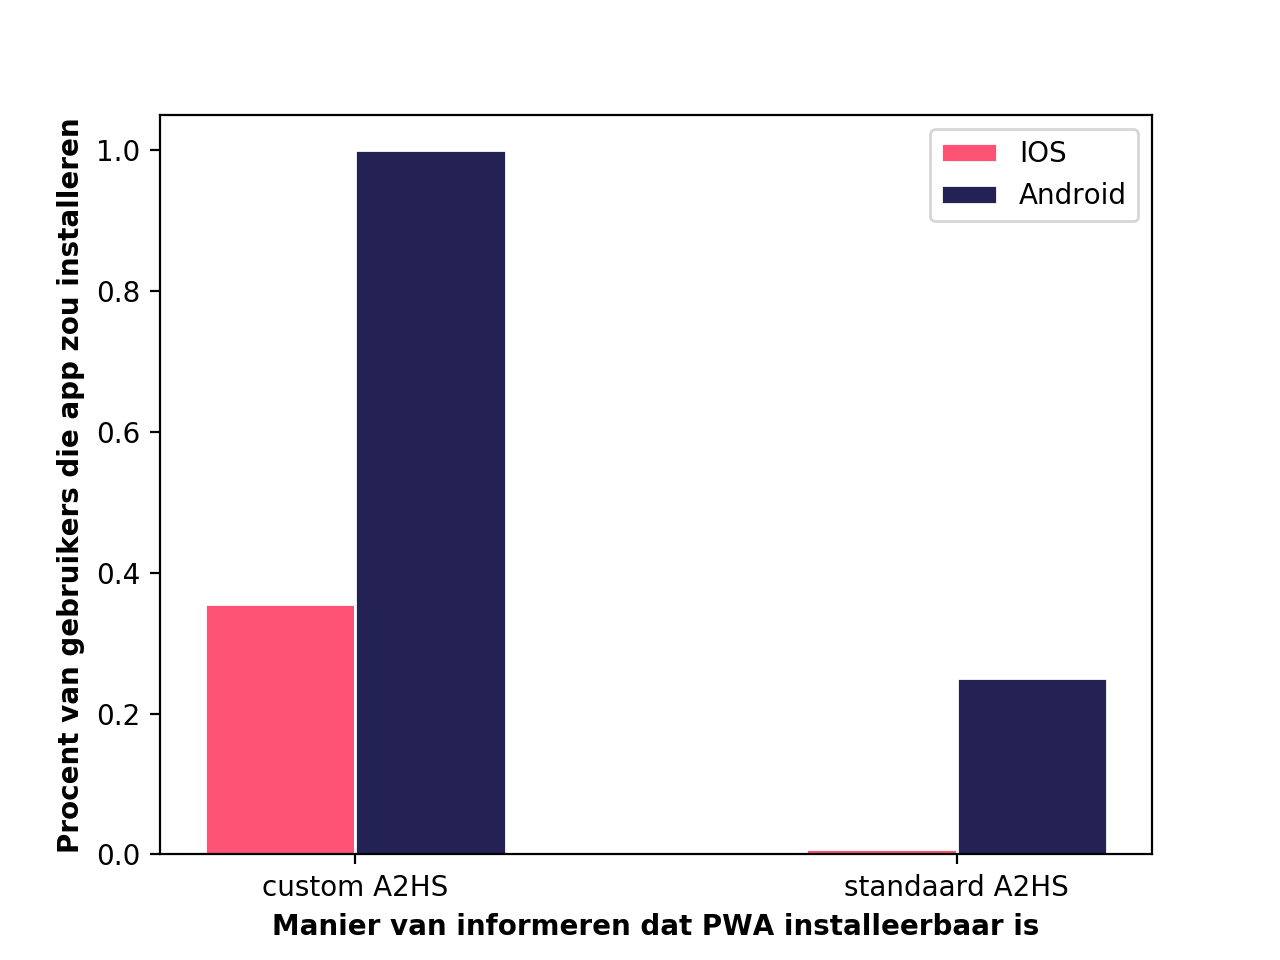
\includegraphics[width=120mm]{./img/A2HS_data.png}
				\caption{A2HS ervaringen}
				\label{fig:A2HSExperience}
			\end{figure}
		
		
	
	\subsection{Native feeling}
		%todo:✅  Vond je de ervaring in de demo's gelijkaardig als die in een mobiele applicatie?
		
		Er werd onderzoek gedaan naar de user experience van een PWA die werd toegevoegd aan het startscherm. Deze applicaties hebben geen browserelementen en zien er dus meer uit als een native applicatie.
		
		
		%todo:📈✅
		De testers kregen de vraag 'Vond je de ervaring in de demo's gelijkaardig als die in een mobiele applicatie?' Hier antwoordde 76,92\% dat ze de ervaring van de PWA's gelijkaardig vonden aan die van een native applicatie.
		
		Ook hier valt op dat de testers die vonden dat de ervaring niet gelijkaardig was aan die van een native applicatie allemaal gebruik maakten van een toestel met iOS als besturingssysteem.
		
	\subsection{Beperkingen van een PWA}
	
		Zoals eerder besproken is de zwakke ondersteuning van PWA-functionaliteiten op Apple-toestellen een grote beperking. Dit is echter niet het enige probleem bij het ontwikkelen van een PWA.
			
		Het is niet eenvoudig om consistent een goeie ervaring te bieden met één codebase voor alle platformen die ondersteund worden. 
		
		Zo werd er beslist om de maximale hoogte van de applicatie vast te zetten op 100vh. Op deze manier is het in principe onmogelijk om een scroll te hebben.
		
		Dit werkte goed op een desktop browser maar gaf problemen op mobiele toestellen.
		
		Op Android bijvoorbeeld maakt de adresbalk geen deel uit van de viewport. Hierdoor was er dus wel een scroll van enkele centimeters aanwezig als de applicatie bezocht werd in de browser. Dit probleem stelt zich niet als de applicatie geïnstalleerd wordt want dan is er geen adresbalk aanwezig.
		

		Er zouden optimalisaties gedaan kunnen worden aan de hand van JavaScript. Ook Ionic zou eventueel een oplossing kunnen bieden. Deze oplossingen verhogen in ieder geval de complexiteit en vallen buiten de scope van dit onderzoek.
	
	
	
	
			
		